% -----------------------------------------------------------------------------------------------------------------------------------------
%
%  Geruest für Arbeiten am Institut für Virtuelle Produktion, ETH Zürich
% -----------------------------------------------------------------------------------------------------------------------------------------
%
% DATEINAME:   arbeit.tex
%
% INHALT:      Hauptdatei fuer Arbeiten
%
% ANWENDUNG:   Mit pdfLaTeX kompilieren
% -----------------------------------------------------------------------------------------------------------------------------------------

\documentclass[11pt,twoside,a4paper,DIV11,numbers=noendperiod]{scrartcl} % Definition des Dokumentenlayouts, Verwendung der KOMA-Klasse scrartcl (aequivalent zum Standardscript article, fuer weitere Informationen siehe: http://www.komascript.de/
\usepackage{ivpthesis_1}                        % Einbinden des IVP-Pakets
\usepackage[english]{babel}                     % Verwendung des deutschen Sprachpakets
\usepackage[left=2.5 cm,right=2.5 cm,top=2.5 cm,bottom=1.7cm,bindingoffset=0.4cm]{geometry} % Angepasste Seitenraender + Offset fuer Bindung
\usepackage[ngerman]{datetime}                  % Datum deutsch
\addtokomafont{caption}{\small}                 % Kleinere Unterschriften
\newdateformat{digitsdate}{\twodigit{\THEDAY}.\twodigit{\THEMONTH}.\THEYEAR} % Datumsformat fuer Titelblatt
\pagestyle{fancy}                               % Definition der Kopfzeile
\setlength{\headwidth}{\textwidth}
\renewcommand{\sectionmark}[1]{\markright{\thesection\ #1}}
\fancyhead{}
\rhead[\nouppercase{\rightmark}]{\thepage}
\lhead[\thepage]{\nouppercase{\rightmark}}
\fancyfoot{}                                   % Definition der Fusszeile
% -----------------------------------------------------------------------------------------------------------------------------------------
% Hier koennen weitere, evtl. benoetigte Pakete hinzugefuegt werden
% -----------------------------------------------------------------------------------------------------------------------------------------
\usepackage{subfigure}                          % Fuer den Gebrauch von subfigures
\usepackage{siunitx}  							% SI-Einheiten
\usepackage[T1]{fontenc}						% Silbentrennung
\usepackage[utf8]{inputenc} 					% Fuer deutsche Umlaute
\usepackage{helvet}                             % Schrift
\renewcommand{\familydefault}{\sfdefault}       % Schrift
\usepackage{booktabs,array}						% for tables
\usepackage{multirow}							% for tables
\usepackage{mathrsfs}
\usepackage[makeroom]{cancel}
\usepackage[colorlinks=false, pdfborder={0 0 0}, bookmarksopenlevel=3,pdfpagelabels=true]{hyperref}% Hyperlinks in PDFs
% -----------------------------------------------------------------------------------------------------------------------------------------
% Nuetzliche Definitionen, koennen nach Belieben erweitert werden
% -----------------------------------------------------------------------------------------------------------------------------------------
\providecommand{\zb}{z.B.}
\providecommand{\ua}{\textit{u.a.}}
\providecommand{\dh}{d.h.}
% -----------------------------------------------------------------------------------------------------------------------------------------
% Typ der Arbeit waehlen
% -----------------------------------------------------------------------------------------------------------------------------------------
%\renewcommand{\ivpthesistype}{Bachelor}
%\renewcommand{\ivpthesistype}{Semester}
\renewcommand{\ivpthesistype}{Master}
% -----------------------------------------------------------------------------------------------------------------------------------------
% Nummer der Arbeit angeben (fuer weitere Information bitte Betreuer oder Frau Haerry (haerry@ivp.mavt.ethz.ch) fragen)
% -----------------------------------------------------------------------------------------------------------------------------------------
\renewcommand{\ivpthesisnumber}{07-001}
% -----------------------------------------------------------------------------------------------------------------------------------------
% Namen von Autoren und Betreuern angeben
% -----------------------------------------------------------------------------------------------------------------------------------------
\renewcommand{\ivpauthor}{Erik Turner}
\renewcommand{\ivpadviser}{Dr. Niko Manopulo\\Dr. Bekim Berisha}
% -----------------------------------------------------------------------------------------------------------------------------------------
% Titelbild
% -----------------------------------------------------------------------------------------------------------------------------------------
% 
% UNBEDINGT LESEN:
% Bild auf der Vorderseite muss ZWINGEND als frontpicture.pdf gespeichert werden! Die Dimension sollte Laenge zu Breite 5:3 betragen.
%
%
% -----------------------------------------------------------------------------------------------------------------------------------------
% Ab hier beginnt das Geruest fuer den Hauptteil der Arbeit
% -----------------------------------------------------------------------------------------------------------------------------------------
\begin{document}
% Alle bib-items werden einbezogen, ohne dass im Text hierauf Bezug genommen wird
%\nocite{*}

% Erster Teil des Vorspanns: Titelseiten, werden nicht nummeriert und auch nicht gezaehlt. Bild wird nicht ins Bilderverzeichnis miteinbezogen.
% Titelseite, Titel der Arbeit eingeben. Falls das Datum (welches mit dieser Einstellung immer das Kompilierdatum ist) geaendert werden muss, soll '\digitsdate\today' durch das entsprechende Datum vom Format DD.MM.JJJJ
\ivptitlepage{Computational material and contact modelling of the interaction between plunger rod and rubber stopper during the assembly of medical syringes}{\digitsdate\today}
\makeatletter
\setlength\@fpbot{0\p@ \@plus 1fil}
\makeatother

% Zweiter Teil des Vorspanns: Seiten werden mit kleinen roemischen Nummern nummeriert. Begonnen wird mit 'i'.
\pagenumbering{roman}

% Erklaerung der Eigenstaendigkeit
\newpage
\addcontentsline{toc}{section}{\protect\numberline{}{Declaration of originality}}
\markright{Eigenständigkeit}
%\section*{Bestätigung der Eigenständigkeit}

%(DEUTSCH/ENGLISCH bitte nicht verwendete Version löschen)


%Ich bestätige, die vorliegende Arbeit selbständig und in eigenen Worten verfasst zu %haben. Davon ausgenommen sind sprachliche und inhaltliche Korrekturvorschläge durch %die Betreuer und Betreuerinnen der Arbeit.
%Ich bestätige mit meiner Unterschrift:
%\begin{itemize}
%\item Ich habe keine im Merkblatt ?Zitier-Knigge? beschriebene Form des Plagiats %begangen.
%\item Ich habe alle Methoden, Daten und Arbeitsabläufe wahrheitsgetreu %dokumentiert.
%\item Ich habe keine Daten manipuliert.
%\item Ich habe alle Personen erwähnt, welche die Arbeit wesentlich unterstützt %haben.
%\item Ich nehme zur Kenntnis, dass die Arbeit mit elektronischen Hilfsmitteln auf %Plagiate überprüft werden kann.
%\end{itemize}


%Ort, Datum:

%\hskip 10pt

%Unterschrift(en):

%\hskip 10pt




\section*{Confirmation of originality}




I hereby confirm that I am the sole author of the written work here enclosed and that I have compiled it in my own words. Parts excepted are corrections of form and content by the supervisor.
With my signature I confirm that
\begin{itemize}
\item 	I have committed none of the forms of plagiarism described in the - Citation etiquette -  information sheet.
\item 	I have documented all methods, data and processes truthfully.
\item 	I have not manipulated any data.
\item 	I have mentioned all persons who were significant facilitators of the work.
\item 	I am aware that the work may be screened electronically for plagiarism.
\end{itemize}



Place, date:

\hskip 10pt

Signature(s):

\hskip 10pt



% Vorwort (optional)
%\newpage
%\addcontentsline{toc}{section}{\protect\numberline{}{Vorwort}}
%\markright{Vorwort}
%\section*{Vorwort}

Einführung und Motivation.

% English and Zusammenfassungen sollen nicht laenger als eine Seite pro Sprache sein.
\newpage
\addcontentsline{toc}{section}{\protect\numberline{}{Zusammenfassung}}
\markright{Zusammenfassung}
\section*{Zusammenfassung}

Zusammenfassung in Deutsch.

\newpage
\addcontentsline{toc}{section}{\protect\numberline{}{Abstract}}
\markright{Abstract}
\section*{Abstract}

Summary in english.


% Verzeichnisse
% Inhaltsverzeichnis
\newpage
\tableofcontents
\addtocontents{toc}{\vspace{.5\baselineskip}}

% Tabellenverzeichnis
\newpage
\addcontentsline{toc}{section}{\protect\numberline{}{List of tables}}
\listoftables

% Abbildungsverzeichnis
\newpage
\addcontentsline{toc}{section}{\protect\numberline{}{List of figures}}
\listoffigures

% Bezeichnungen
\newpage
\addcontentsline{toc}{section}{\protect\numberline{}{Nomenclature}}
\addtocontents{toc}{\vspace{.5\baselineskip}}
\markright{Nomenclature}
\section*{Nomenclature}
\label{s:Bezeichnungen}

\begin{table}[!htb]
	\centering
    \def\arraystretch{1.5}
		\begin{tabular}{l p{10cm}}
	 \hline
     Abbreviation & Meaning \\
	  \hline
		PFS & Pre-Filled Syringe \\
		
		PS & Plunger Stopper \\
        
        PR & Plunger Rod \\
        
        GB & Glass Barrel \\
        
        CPP & Critical Process Parameters \\
        
        CQA & Critical Quality Attributes \\
        
        CMA & Critical Material Attributes
		\end{tabular}
	\caption{List of abbreviations}
	\label{tab:bezeichnungen}
\end{table}


% Ab hier beginnt die eigentliche Arbeit. Seiten werden arabisch nummeriert, beginnend mit '1'.

\clearpage
\pagenumbering{arabic}

% Introduction
\newpage
%\addcontentsline{toc}{section}{\protect\numberline{}{Introduction}}
%\addtocontents{toc}{\vspace{.5\baselineskip}}
\markright{Introduction}
\section{Introduction}
\subsection{Motivation}
The idea for this thesis was developed during my internship in 2017 at the Device Development
Department of F. Hoffmann-La Roche. There, I was working in the Process Engineering group whose main responsibility is to implement the design transfer. Design transfer means in simple terms translating the device design into manufacturing specifications by developing the production process. An important step for this is the process design which consists of the combination of a risk assessment and process design studies. The objective is to understand the process by characterizing its critical process parameters (CPPs), critical quality attributes (CQAs), critical material attributes (CMAs), proven acceptable ranges (PARs) and key performance indicators (KPIs). These studies require generally a lot of time, material costs, occupation of the production lines and deliver sometimes insufficient data as soon as there is a slight product change. My motivation thus was to enable more production flexibility and productivity through an improved development process. In order to do this, I was set to implement engineering tools and concepts to a real project study such as Design of Experiments (DoE) and Finite Element Analysis (FEA) to leverage a more thorough process understanding. Furthermore, my aim is to show the potential of this approach and to add it to the  group toolbox.

The practices mentioned above are often used as lean manufacturing tools. Some of them were initially developed by the automobile industry for process improvement purposes and are today increasingly being adopted by the pharmaceutical industry driven by the need to reduce manufacturing costs and increase productivity. One of the main manifestations of this phenomenon is the Quality by Design (QbD) initiative supported mainly by the Food and Drug Administration (FDA) through the International Council for Harmonisation of Technical Requirements for Pharmaceuticals for Human Use (ICH). 
 In these guidelines, a set of practices, including DoE and mechanistic models are recommended as useful tools for process development activities. The challenge consists in being able to take the relevant tools from the lean practices and adapting them for their needs rather than just copying them.
Ultimately, the correct implementation of these tools has the potential to reduce process variability, increase quality and to finally leverage more robust processes. 

\begin{figure}[h!]	
	\centering
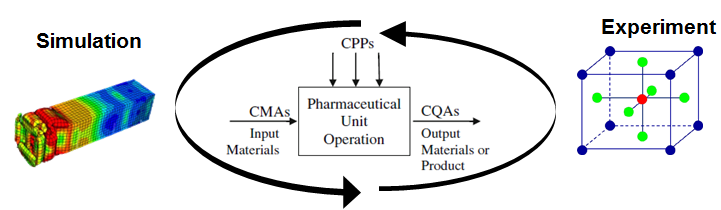
\includegraphics[height=4cm]{img/DesignSpace.PNG}
   \caption{The combination of designed experiments and simulation yields process understanding and finally the design space.}
 \label{fgr:PFS}
\end{figure}
\newpage
\subsection{Research}

\subsubsection{Background}
During the final assembly of pre-filled medical syringes, a polymer rod is snapped into the
rubber stopper, which in turn provides isolation of the liquid medical agent. The resistance
necessary for the snap-in to occur is on the one hand provided by the air pressure compressed between liquid and rubber stopper, and on the other through friction of the stopper with the surrounding glass container. The former is caused by stopper downward movement and it is triggered by a lower break loose force (static friction between the glass barrel internal wall and the stopper) than the pushing plunger rod insertion force. The displacement represents a quality risk to the product as it has the potential to pull contaminants into the drug product but also to further compromise additional component assembly, packaging and finally the patient. The objective is thus to mitigate the risk by minimizing the displacement to assure product conformity to specifications. 
From a computational point of view, this is a challenging problem due to several reasons. Rubber materials mostly obey hyperplastic constitutive relations and thus require FEM formulations able to deal with volumetric locking effects. Furthermore, the snap-in problem itself represents an instability state, which is known to cause convergence issues, which are further deepened by the loosely defined friction conditions.

\subsubsection{Objective}
The primary goal of this thesis is the development of a robust and validated computational
model able to deal with the mentioned challenges and to deliver sufficient accuracy. This will enable the quantification of the plunger stopper displacement for defined process parameters and thus to determine if the product is within the specification or not.
Furthermore, this thesis it is aimed to design a set of real/virtual experiments in order to elucidate the effect of the different factors influencing the process and determine the operating range of the process parameters.

\subsubsection{Methodology}
As mentioned in the background, this work is based on a combination of simulation and experiments. The starting point is the simulation of the assembly process with a representative 2D axisymmetric static model with nominal component specifications. As there are two relative movement phenomena: plunger rod insertion and stopper movement, each are modeled separately at first in order to calibrate the model. In a later stage, the whole process is simulated and then validated with experiments to test the model accuracy. This is then repeated for a dynamic simulation. The second phase involves sensitivity analysis and is performed in order assess the most critical contributing factors to the snap-in. Designed experiments also serve as validation tool for selected factors.

\newpage
\subsection{Outline}
The thesis is organized as follows. First, an introduction is given in the 1st chapter with the motivations, objectives and context of this work. Then, relevant literature is presented and analyzed in the 2nd chapter first in the context of pre-filled syringes and secondly, for finite element related problems with emphasis on hyperelastic, contact and instability modeling.
Afterwards the theoretical framework of process modelling in chapter 3 and then of finite element modeling is exposed. Specifically, the basics of nonlinear, hyperelastic, contact modeling are explained in the chapters 4, 5 and 6. 
The 7th chapter illustrates  the input data used for ANSYS is including the material data generation and the CAD geometry. 
Then, some initial considerations are given regarding the physics and the important parameters of the assembly process in chapter 8. Afterwards, the results of the FE analysis  for both the static and dynamic cases are exposed and discussed in conjunction with the validation experiments in chapter 9. A critical inflection is given on the validity on the model and put in context with the results of sensitivity analysis. Chapter 10 illustrates the obtained experimental results from the experimental design and statistical results.
Finally, the conclusion and an outlook are given in chapter 11.



% Literature
\newpage
%\addcontentsline{toc}{section}{\protect\numberline{}{Introduction}}
%\addtocontents{toc}{\vspace{.5\baselineskip}}
\markright{literature analysis}
\newpage
\part{Theory section}
In this first theory part the basis of finite element modeling will be laid out, including some basic founding notions of non-linear FEM in chapter 3 then in chapter 4 hyperelastic material models followed by contact modeling in chapter 5. Finally and overview in how metamodels can be used and implemented is given in chapter 6.
\section{Literature analysis}
A lot is done in industry
\subsection{Finite element analysis}
\subsection{Pre-filled syringes}








% Process modelling
\newpage
%\addcontentsline{toc}{section}{\protect\numberline{}{Design, Optimization and Robustness Analysis}}
%\addtocontents{toc}{\vspace{.5\baselineskip}}
\markright{Design, Optimization and Robustness Analysis}
\newpage
\section{Process modeling}
\subsection{Process components}
Operator -> Equipment <-> Material-> Part


A Manufacturing Process is a Changein the Workpiece Material
•A change in geometry
•A change in constitutive properties

There is an energy transfer occurring: mechanical, electrical, thermal or chemical 


\subsubsection{Variability}
Control of variation: identify, characterize, minimize.

Deterministic
Random: measure with probability, statistics, predict

Manufacturing: Quality, Rate, Cost, Flexibility
Quality: conformance to specifications => minimize variability

Deterministic: equipment, material, operation
Random: probabilistic model of the process, Statistics as output, Deviation from expected behaviour
Variation reduction, factors influencing statistical behaviour, optimization of statistical behavior
Sources: material, equipment, operator and environment

\begin{table}[!htb]
	\centering
    \def\arraystretch{1.5}
		\begin{tabular}{l l l}
	 \hline
      & States & Properties \\
	  \hline
		Material & & \\
		
		Equipment & & 
		\end{tabular}
	\caption{Process Parameters}
	\label{tab:bezeichnungen}
\end{table}

\begin{equation}
\Delta Y=\frac{\partial Y}{\partial \alpha}\Delta \alpha + \frac{\partial Y}{\partial u}\Delta u 
\end{equation}

With $\frac{\partial Y}{\partial \alpha}$ Disturbance Sensitivity, $\Delta \alpha$ Disturbances, $\frac{\partial Y}{\partial u}$ Control Sensitivity and $\Delta u$ Control Inputs.

Disturbances are reduced with standard operating procedures (SOPs) and Statistical analysis and identification of variation sources (SPC). The sensitivity of the disturbances are reduces with designed experiments to measure the sensitivity and thus make the process robust. Finally the more direct approach is to measure the output and manipulate the input with the so-called feedback control. Here under are schematically depicted the three methods 

\begin{figure}[h]
\centering
  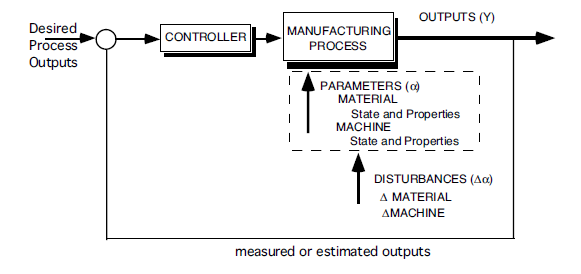
\includegraphics[height=4cm]{img/directfb.PNG}
   \caption{adaptive mesh generation}
 \label{fgr:graft}
\end{figure}





\begin{enumerate}
\item Physical Model
\item Empirical Model
\item Statistical Model
\end{enumerate}


Variation Equation
Reduce Disturbances (Statistical Analysis)
Reduce Senstivity (optimization \& robustness)


 Design, Optimization and Robustness Analysis

\subsection{Experimental design}
\subsubsection{ANOVA}
\subsubsection{Design of Experiments (DoE)}
Correlation
Regression
Full Factorial
Taguchi


\subsection{Metamodeling}
Study Physics of Process
–Define Important Inputs
–Intuition about model
–Limits on inputs
•Define Optimization Penalty Function
–J=f(x)


Procedure
•Identify model (linear, quadratic, terms to include)
•Define inputs and ranges
•Identify “noise”parameters to vary if possible ($\Delta \alpha$’s)
•Perform Experiment
–Appropriate order
•randomization
•blocking against nuisance or confounding effects


Solve for $\beta$’s
•Apply ANOVA
–Data significant?
–Terms significant?
–Lack of Fit Significant?
•Drop Insignificant Terms
•Add Higher Order Terms as needed
Search for Optimum
–Analytically
–Piecewise
–Continuously
Find Optimum value x*
•Perform Confirming experiment
–Test Model at x*
–Evaluate error with respect to model
–Test hypothesis that
y(x*)=ˆ y (x*)
If hypothesis fails
–Consider new ranges for inputs
–Consider higher order model as needed
–Boundary may be optimum!

Procedure for DOE/OptimizationFor

Study Physics of Process–Define important inputs–Intuition about model–Limits on inputs•DOE–Factor screening experiments–Further DOE as needed–RSM Construction•Define Optimization/Penalty Function–J=f(x)


(1) DOE Procedure


•Identify model (linear, quadratic, terms to include)
•Define inputs and ranges
•Identify “noise”parameters to vary if possible ($\Delta \alpha$’s)
•Perform experiment
–Appropriate order
•randomization
•blocking against nuisance or confounding effects

(2) RSM Procedure


•Solve for $\beta$’s
•Apply ANOVA
–Data significant?
–Terms significant?
–Lack of Fit significant?
•Drop Insignificant Terms
•Add Higher Order Terms as needed


(3) Optimization Procedure


•Define Optimization/Penalty Function
•Search for Optimum
–Analytically
–Piecewise
–Continuously/evolutionary
•Confirm Optimum




% Finite Elements Model
\newpage
%\addcontentsline{toc}{section}{\protect\numberline{}{Finite Element Modeling}}
%\addtocontents{toc}{\vspace{.5\baselineskip}}
\markright{Non-linear Finite Element Modeling}


\newpage
\section{Nonlinear FEM}
\label{s:Finite Element Modeling}

In this chapter the theory of FEM will be laid out.
The finite element method is a numerical technique used to obtain approximate solution to partial differential equations (PDEs) that represent physical problems. There are several techniques to obtain the approximate solution of PDEs. Some of the popular methods are:
\begin{enumerate}
\item Finite Difference Method (FDM)
\item Finite Volume Method (FVM)
\item Finite Element Method (FEM)
\item Boundary Element Method (BEM)
\item Spectral Method
\item Perturbation Method
\end{enumerate}
The main advantage of FEM consists of being able to deal with complex boundaries.
\subsection{Introduction to FEM}
The main steps of the solution process are indicated in the following picture
\begin{figure}[h]
\centering
  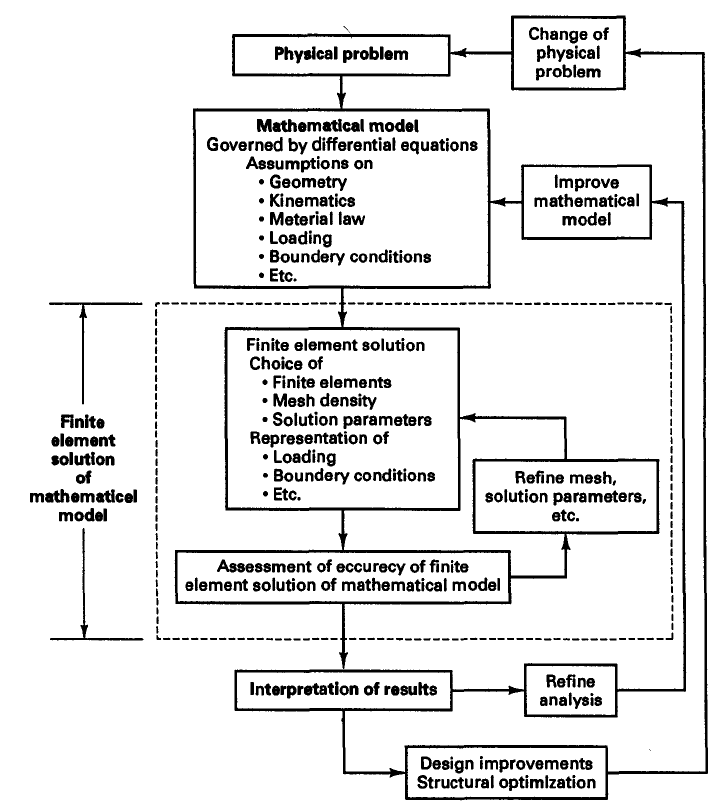
\includegraphics[height=12cm]{img/procedure.png}
   \caption{FEM process workflow.}
 \label{fgr:graft}
\end{figure}
In a first pre-processing phase you describe the problem: simplify a real engineering problem into a problem that can be solved by FEA. Then you discretized/mesh the solid, define material properties, apply boundary conditions.
Then you choose the processing conditions: approximate functions, formulate linear equations, and solve equations.
Finally, in the post-processing you obtain, visualize and explain the results.
\begin{enumerate}
\item Problem Formulation\\
The formulation of the specific governing the response of a system under specific loads and constraints at its boundaries is usually provided in the form of a differential equation. The differential equation is known as the \textit{strong form} of the problem and it includes
\begin{itemize}
\item Conservation of mass, momentum, energy
\item A measure of deformation, often called a strain-dispacement equation
\item A constitutive equation, which describes material behavior and relates stress to a measure of deformation
\end{itemize}
The following set of equations are a simple example:
\begin{align}
&\textrm{Equilibrium Equations:} &f(x)&=R+\frac{aL+ax}{2}(L-x)\\
&\textrm{Constitutive Requirements:}& \sigma&=E\epsilon\\
&\textrm{Kinematics Relationships:}& \epsilon&=\frac{du}{dx}
\end{align}
\item Discretization/Meshing\\
The continuum is discretized using a mesh of finite elements. These elements are connected at nodes located on the element boundaries.
\item Interpolation -The Shape Functions\\
The state of deformation, stresses, etc. in each element is approximated by a the set of corresponding values in the nodes; these nodal values are the basic unknowns of the MFE. Values between nodes, have to therefore result via interpolation.
\item 
\end{enumerate}


Three main methods exist when dealing with a FEM problem approximation: direct, variational and weighted residual method.
The direct approach is related to the “direct stiffness method” of structural analysis and is used for the analysis of discrete systems. For continuous and more complex  however, we have to use the other methods.
Continuous systems describe the physical behavior as a collection of infinitesimal material points(continuum).
Instead of enforcing equilibrium on the discrete system components, differential elements are used.
This results in a set of differential equations called strong form with the accompanying boundary conditions (essential and natural). 
These systems can be «discretized» and thus converted to discrete systems and be solved as in the direct solution.

The solution requires the following steps:
\begin{enumerate}
\item Discretization/idealization of the system into finite elements
\item Equilibrium relations with the element stiffness matrix
\item Determination of the stiffness properties
\item Build system of global algebraic equations
\item Determination of boundary conditions
\item Solve sequence: evaluation of degrees of freedom and response of each element 
\end{enumerate}

However in this differential approach the analytical solution is to difficult to evaluate because of complex geometries, loadings and boundary conditions.
Thus, instead of trying to solve the problem analytically, we would like to do it in an approximate, i.e., numerical way.
To this end, let us first consider what are the possible ways in which the system is allowed to deform. However in order to do it correctly we must check which are the kinematically admissible ways for the system to deform from a state $u(x)$ to a state $u(x)+\delta u(x)$. This is the case if:
\begin{enumerate}
\item $u(x)$ and $u(x)+\delta u(x)$: are continuous over the domain, \textit{i.e.} $u(x)  \in C_o \textrm{in} x \in [0, L]$
\item satisfy exactly the displacement BC, \textit{i.e.} $u(0)=0.$
\end{enumerate}

\begin{figure}[h]
\centering
  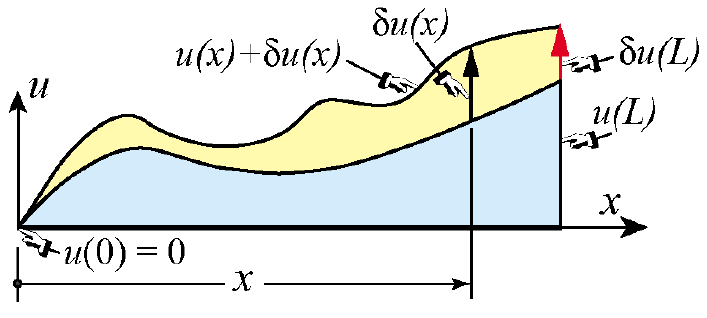
\includegraphics[height=5cm]{img/kinematic.png}
   \caption{Admissible displacements of $\delta u(x)$.}
 \label{fgr:graft}
\end{figure}
\subsubsection{Principle of Virtual Work}
The true deformation $u^*(x)$ is the one satisfying the principle of virtual work. The virtual work of a system of equilibrium forces vanishes when compatible virtual displacements $\delta u(x)$ are imposed:
\begin{equation}
\underbrace{	\int_{\Omega}\underline{\underline{\delta\epsilon}}:\underline{\underline{\sigma}} d\Omega
\rule[-12pt]{0pt}{5pt}}_{\mbox{Internal work}}
=
\underbrace{	\int_{\Omega}\delta u^{T} \cdot f^{B}d\Omega \rule[-12pt]{0pt}{5pt}}_{\mbox{Body forces (gravity)}}
+ 
\underbrace{	\int_{\Gamma}\delta u^{T} \cdot f^{S}d\Omega \rule[-12pt]{0pt}{5pt}}_{\mbox{Surface reactions}}
+ 
\underbrace{	\sum_{i}\delta u \cdot R_{C}^{i}			\rule[-12pt]{0pt}{5pt}}_{\mbox{Point loads}}
\end{equation}

With $\delta \vec{u}$ as Virtual Displacement must satisfy $ \vec{u}_r$ on $\Gamma_u$ and $\boldsymbol{\sigma}$ stress tensor and $\boldsymbol{\delta \epsilon}$ which is a function $\delta \vec{u}$.  
For elastic systems subject to conservative forces (which is the case of systems we are dealing with), the principle of Virtual Work is equivalent to principle of minimum total potential energy (MPE).
The MPE principle states that the actual displacement solution u*(x), out of possible trial solutions, that satisfies the governing equations is the one which renders the Total Potential Energy functional $\Pi$ stationary:
\begin{equation}
\delta \Pi = \delta U - \delta W=0 if u0u^*
\end{equation}
With U being internal energy (strain energy) and W external work.
If we assume $R^i_C$ is integrated into $\boldsymbol{f}^{\Gamma}$ it's equal to zero.

Given:
\begin{align*}
\boldsymbol{u}		&=\boldsymbol{H\hat{u}} & \boldsymbol{\delta u }	&=\boldsymbol{H\delta\hat{u}} & \boldsymbol{\sigma=C:\epsilon} \\
\boldsymbol{\epsilon}&=\boldsymbol{B\hat{u}} & \boldsymbol{\delta \epsilon}	&=\boldsymbol{B\delta\hat{u}=\delta\hat{u}^T B^T}
\end{align*}

Into the equation gives:
\begin{equation}
\int_{\Omega}\delta \boldsymbol{\hat{u}}^T\boldsymbol{B^TCB}\boldsymbol{\hat{u}} d \Omega
=
\int_{\Omega}\delta \boldsymbol{\hat{u}^{T}  H^{B} f^B } d\Omega 
+ 
\int_{\Gamma}\delta \boldsymbol{\hat{u}^{T}  H^{B} f^{\Gamma} } d\Gamma
\end{equation}

Arbitrary simplification of $\delta \textbf{u}$.
\begin{equation}
\underbrace{	\int_{\Omega} \boldsymbol{B^TCB}\boldsymbol{\hat{u}} d \Omega \rule[-12pt]{0pt}{5pt}}_{\mbox{\textbf{K} Stiffness matrix}}
=
\underbrace{	\int_{\Omega}\boldsymbol{H^{B} f^B } d\Omega \rule[-12pt]{0pt}{5pt}}_{\mbox{$\boldsymbol{F}^T$ Body force vector}}
+ 
\underbrace{	\int_{\Gamma} \boldsymbol{ H^{B} f^{\Gamma} } d\Gamma \rule[-12pt]{0pt}{5pt}}_{\mbox{$\boldsymbol{F}^S$ Body force vector}}
\end{equation}

Thus with the following:
\begin{align*}
\boldsymbol{K}&=\int_{\Omega} \boldsymbol{B^TCB}\boldsymbol{\hat{u}} d \Omega &	\boldsymbol{F}^B&=\int_{\Omega}\boldsymbol{H^{B} f^B } d\Omega & \boldsymbol{F}^S&=\int_{\Gamma} \boldsymbol{ H^{B} f^{\Gamma} } d\Gamma
\end{align*}
Yields:
\begin{equation}
\boldsymbol{K \hat{u}= F^B + F^S + \sum_{i} R_{C}^{i}= F}
\end{equation}


Discretized FEM equations:
\begin{equation}
\boldsymbol{K^{el} \hat{u}^{el}= F^{el}}
\end{equation}
These integrals must be computed in each element. This is mostly done numerically. Therefore elements have so-called "integration points"
\begin{equation}
\int f(\vec{x})d\vec{x}=\sum_{i=1}^{N_i}w_if_i
\end{equation}

\subsubsection{Weighted Residuals Method}
Weighted residual method (WRM) is a class of method used to obtain the approximate solution
to the differential equations of the form. It starts with an estimate of the the solution and demand that its weighted average error is minimized

\begin{equation}
\label{eq: diff}
\mathscr{L}(\phi) +f=0 \quad \textrm{in} \quad D
\end{equation}
It involves two major steps. In the first step, we assume an approximate solution
based on the general behavior of the dependent variable. It is selected to satisfy the boundary conditions for f. The assumed solution is then substituted in the differential equation. Since the assumed solution is only approximate, it does not satisfy the differential equation resulting in an error or what we call a residual. The residual is then made to vanish in some average sense over the entire solution domain. This procedure results in a system of algebraic equations. The second step is to solve the system of equations resulting from the first step subject to the prescribed boundary condition to yield the approximate solution sought.
Let $\psi(x) \approx \phi(x)$  be an approximation of the differential equation \ref{eq: diff}. When this is done it is unlikely that the equation is satisfied, thus $R(x)$ is a measure of error called \textit{residual}.
\begin{equation}
\label{eq: sub}
\mathscr{L}(\psi) +f=R
\end{equation}
If the equation \ref{eq: diff} is multiplied by an arbitrary \textit{weight function} and integrated over the domain $D$
\begin{equation}
\int_D w[\mathscr{L}(\phi) +f]dD=0 
\end{equation}
The equations are equivalent. Now, substituting for $\psi$ yields:
\begin{equation}
\label{eq: eq}
\int_D w(x)[\mathscr{L}(\psi) +f]dD=\int_D w(x)R(x) +f]dD \neq 0 
\end{equation}
The integral in \ref{eq: eq} gives the weighted average of the residual over the solution domain. In weighted residual method we force this integral to vanish over the solution domain. That is,
\begin{equation}
\int_D w(x)R(x)dD=0 
\end{equation}
In the form of a generalized Fourier series the function can be approximated as following:
\begin{equation}
\psi(x)=\sum_{i=1}^nc_iN_i(x)=c_1N_1(x)+c_2N_2(x)+...+c_nN_n(x)
\end{equation}
In vector form
\begin{equation}
\boldsymbol{\psi(x)=C^TN^T=(NC)^T=NC}
\end{equation}
Where \textbf{N} is the row vector 
\begin{equation}
\boldsymbol{N}=
\begin{matrix}
[ N_1	& N_2 & ... & N_n ]
\end{matrix}
\end{equation}
And \textbf{C} is the column vector 
\begin{equation}
\boldsymbol{C}=\left[
\begin{matrix}
C _1	\\ C_2 \\ ... \\ C_n 
\end{matrix} \right]
\end{equation}
Here $ci$’s are unknown coefficients called\textit{ fitting coefficients} and $n$ is the number of fitting coefficients. $N_i(x)$’s are assumed to be linearly independent functions of x and are called \textit{trial functions}.
The trial functions can be polynomials, trigonometric functions etc. The trial functions are usually chosen in such a way that the assumed function $\psi(x)$ satisfies the global boundary conditions for $\phi (x)$, although this not strictly necessary and certainly not always possible.

Polynomial Approximation. One of the simplest choices for a trial function is a polynomial, for a one-dimensional problem which can be obtained by taking $N_i(x) = x^i$. The result is
\begin{equation}
\psi(x)= \sum_{i=0}^nc_ix^i=c_0+c_1x+...+c_nx^n
\end{equation}
This produces a smooth solution, but it suffers the same limitations as Lagrange interpolation. A particularly significant flaw is that this choice need not converge to $\phi(x)$ as $n$ increases.
With the selection of $\psi(x)$ as the series expansion (4.6), it is evident that the residual $R$ depends on the unknown parameters $c_i$’s in the expansion:
\begin{equation}
R=R(x;C)
\end{equation}
If the number of trial functions n is sufficiently large, then in principle, the unknown parameters $ci$’s can be chosen so that the residual $R$ is small over the domain.
Weight functions. In general the weight function $w(x)$ may be written as
\begin{equation}
w(x)= \sum_{i=0}^na_iw_i=a_1w_1+a_2w_2+...+a_nw_n=\boldsymbol{aw}
\end{equation}
Where \textbf{a} and \textbf{w} are respectively the row  and the column vectors
\begin{equation}
\boldsymbol{a}=
\begin{matrix}
[ a_1	& a_2 & ... & a_n ],
\end{matrix} 
\quad 
\boldsymbol{w}=\left[
\begin{matrix}
w _1	\\ w_2 \\ ... \\ w_n 
\end{matrix} \right]
\end{equation}
Here $wi$’s are known functions of x and ai’s are constant parameters. Substituting $w(x) = \boldsymbol{aw}$ in
the weighted residual equation (4.5) to yield
\begin{equation}
\boldsymbol{a\int_Dw}RdD=0
\end{equation}
Since \textbf{a} is a constant vector, we have
\begin{equation}
\boldsymbol{\int_Dw}RdD=0
\end{equation}or
\begin{align}
\boldsymbol{\int_Dw_1}RdD=0\\
...\\
\boldsymbol{\int_Dw_n}RdD=0
\end{align}
Now we have $n$ equations to determine unknown coefficients $ci$’s. Finally, inserting $\psi = \boldsymbol{NC}$ in
equation \ref{eq: sub} yields
\begin{equation}
R=\mathscr{L}(\boldsymbol{NC})+f=\mathscr{L}\boldsymbol{(N)C}+f
\end{equation}
and hence the 
\begin{equation}
\left[\int_D \boldsymbol{w}\mathscr{L}(\boldsymbol{N})dD\right]\boldsymbol{C}=-\int_D\boldsymbol{w}fdD
\end{equation}
Introduction matrix \textbf{K} and \textbf{f }as
\begin{equation}
\boldsymbol{K}=\int_D \boldsymbol{w}\mathscr{L}(\boldsymbol{N})dD, \quad \boldsymbol{f}=-\int_D\boldsymbol{w}fdD
\end{equation}

allows us to write the equation in compact form 
\begin{equation}
\boldsymbol{KC=f}
\end{equation}
The system of equations can be solved for n unknown coefficients $ci$’s provided that a suitable weight function $w$ is selected.
With regards to the selection of weight function, we have several choices. Hence, depending
upon nature of weight function, we have different types of weighted residual methods. Some of
the standard methods are:
\begin{enumerate}
\item Point Collocation Method
\item  Subdomain Collocation Method
\item  Least Square Method
\item  Galerkin Method
\end{enumerate}

\paragraph{Galerkin Method}
In Galerkin version of weighted residual method, the weight functions are chosen to be the trial
functions themselves. This is the method we usually used for developing finite element equations
for field problems. So, in Galerkin method we set
\begin{equation}
w_i=N_i \quad (i=1,2,...,n)
\end{equation}
The unknown coefficients in the approximate solution are determined by setting the integral
over D of the weighted residual to zero. For one-dimensional problem in the interval [a,b], this
procedure will results
\begin{equation}
\int_a^bw_iR(x)dx=\int_a^bN_iR(x)dx=0
\end{equation}Following points about Galerkin method may be noted:
• Galerkin method produces symmetric positive definite coefficient matrix if the differential
operator is self-adjoint.
• Galerkin method requires less computational effort compared to the least square method.
\subsubsection{Variational Method}
In this approach the physical problem is restated using the aforementioned principle of minimum potential energy. This variational form is also know as the weak form and it is widely used for deriving finite element equations whenever classical variational statement is available for the given problem. For approximate solutions, a larger class of trial solutions $u(x)$ can be employed than in the differential formulation; for example, the trial functions do not need to satisfy the natural BC because these are implicitly contained in the functional. The approximation is based on the minimization of the functional.
The major drawback of this approach is that it's not useful for nonlinear problems . 
The Rayleigh-Ritz method is an approximate method based on the variational formulation.
If you consider a PDE with variational structure the variational form of 
\begin{equation}
I(u)=\int_{\Omega}[\frac{k}{2}\left(\frac{\partial u}{\partial x_1}\right)^2+\frac{k}{2}\left(\frac{\partial u}{\partial x_2}\right)^2 +fu]d\Omega
\end{equation}
\paragraph{Rayleigh-Ritz Method}
Rayleigh–Ritz method replaces the trial functions into the functional (variational) form of the PDE. It's advantageous since less differentiability is required and the natural boundary conditions are already in the function. Hence, there is no need for the trial functions to satisfy them.
\begin{equation}
\hat{u}=\sum_{i=1}^nw_if_i\cong u(x)
\end{equation}
Thus the functions $f_i$ only need to be differentiable once and it only needs to satisfy $u_0=0$



\subsubsection{Isoparameteric Continuum Elements}
In general, we would like to be able to represent any element in a standardized manner –introducing a transformation between a set of standardized (natural) coordinates and the real (global) coordinates
Different schemes exist for establishing such transformations: isoparametric representations (same nodes for both geometry and displacement representation)
Displacement fields as well as the geometrical representation of the finite elements are approximated using the same approximating functions –shape functions. This transformation allows us to refer to similar elements (eg. truss, beams, 2D elements, in a standard manner, using the natural coordinates (r,s), without every time referring to the specific global coordinate system (x,y).
Isoparametric elements can be one-, two-or three-dimensional:

The principle is to assure that the value of the shape function hiis equal to one in node iand equals zero in other nodes.

In order to establish the stiffness matrixes we must differentiate the displacements with respect to the coordinates (x, y, z). Since the shape functions are usually defined in natural coordinates we must introduce the necessary coordinate transformation between natural and global or local coordinate system. For example in the 3D domain we can express the derivative of a function which is expressed in terms of coordinates (x,y,z), with respect to an other set of coordinates (r,s,t) as:


\paragraph{Shape Function}
Shape functions will be defined as interpolation functions which relate the variables in the finite element with their values in the element nodes. The latter are obtained through solving the problem using finite element procedures.
Regardless of the dimension of the element used, we have to bear in mind that Shape Functions need to satisfy the following constraints:
\subsection{Continuum mechanics}
In case of linear deformation the reference and current configurations coincide.
For large deformations the difference is important. The reference configuration is independent of time, this means a reference point will always correspond to a material particle, hence \textit{material configuration}. This is also denoted as \textit{Lagrangian Configuration} as it is from the Lagrangian viewpoint. On the other hand the point in the current configuration do not correspond to the material points, but to the points in space. This is denoted \textit{spatial configuration} and corresponds the a material flow through a fixed domain as postulated by the Eulerian viewpoint, hence \textit{Eulerian Configuration}.
The differences between Lagrangian and Eulerian meshes are most clearly seen in terms of the behavior of the nodes. If the mesh is Eulerian, the Eulerian coordinates of nodes are fixed, i.e. the nodes are coincident with spatial points. If the mesh is Lagrangian, the Lagrangian material coordinates X of nodes are time invariant, i.e. the nodes are coincident with material points.
\begin{figure}
\centering
  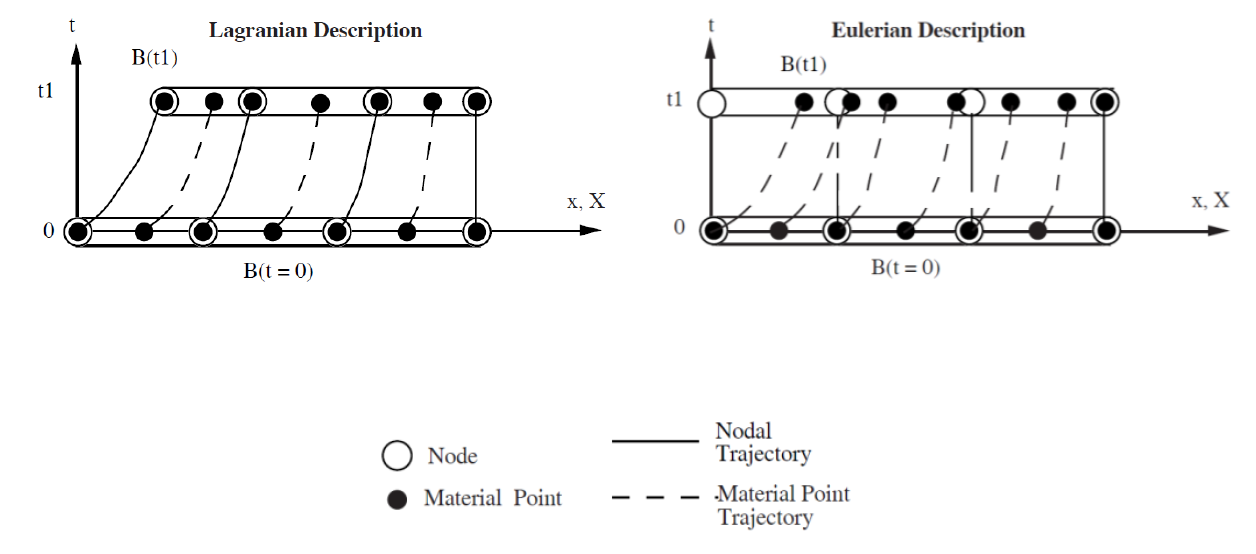
\includegraphics[height=4cm]{img/ale.png}
   \caption{Space time depiction of a one dimensional Lagrangian, Eulerian and ALE (arbitrary Lagrange Eulerian) element.}
 \label{fgr:graft}
\end{figure}
In the Eulerian mesh, the nodal trajectories are vertical lines and material points pass across element interfaces.
In the Lagrangian mesh, nodal trajectories are coincident with material point trajectories, and no material passes between elements. Furthermore,
element quadrature points remain coincident with material points in Lagrangian meshes, whereas in Eulerian meshes the material point at a given
quadrature point changes with time. We will see later that this complicates the treatment of materials in which the stress is history-dependent. In Lagrangian meshes, since the material points remain coincident with mesh points, the elements deform with the material. Therefore, elements in a
Lagrangian mesh can become severely distorted. This effect is apparent in a onedimensional problem only in the element lengths: in Eulerian meshes, the
element length are constant in time, whereas in Lagrangian meshes, element lengths change with time. In multi-dimensional problems, these effects
are far more severe, and elements can get very distorted. Since element accuracy degrades with distortion, the magnitude of deformation that can be
simulated with a Lagrangian mesh is limited. Eulerian elements, on the other hand, are unchanged by the deformation of the material, so no degradation in accuracy occurs because of material deformation.
The comparative advantages of Eulerian and Lagrangian meshes can be seen even in this simple one-dimensional example. Since the nodes are
coincident with material points in the Lagrangian mesh, boundary nodes remain on the boundary throughout the evolution of the problem. This
simplifies the imposition of boundary conditions in Lagrangian meshes.
In Eulerian meshes, on the other hand, boundary nodes do not remain coincident with the boundary. Therefore, boundary conditions must be imposed at points which are not nodes, and as we shall see later, this engenders significant complications in multi-dimensional problems. Similarly, if a node is placed on an interface between two materials, it remains on the interface in a Lagrangian mesh, but not in an Eulerian mesh.

\begin{figure}
\centering
  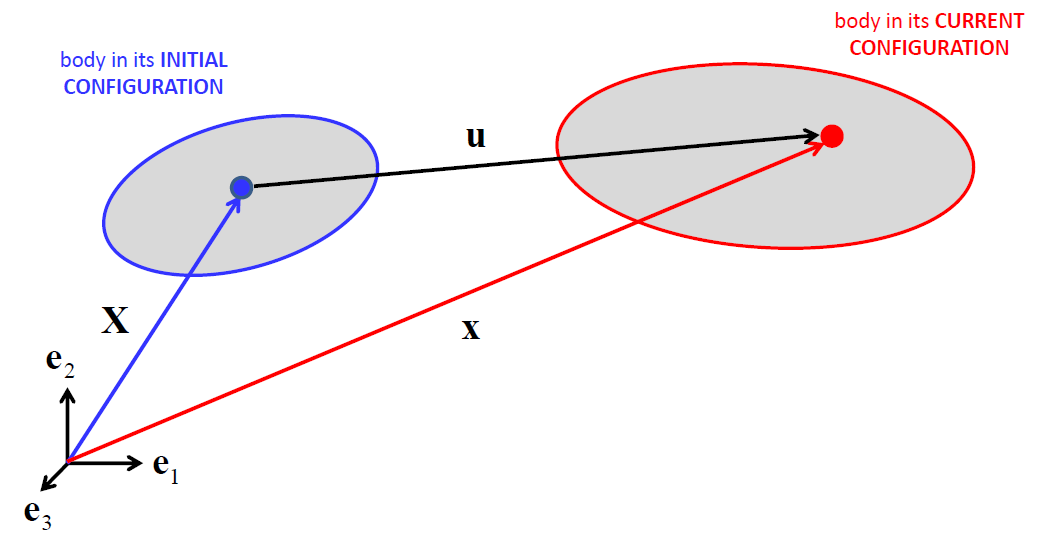
\includegraphics[height=6cm]{img/Def.png}
   \caption{adaptive mesh generation}
 \label{fgr:graft}
\end{figure}
Displacement:
\begin{equation}
u=x-X
\end{equation}

\begin{align}
&\textrm{Reference configuration:}& u(X,t)&=\phi(X,t)-X \\
&\textrm{Current configuration:}& u(x,t)&=x-\phi^{-1}(x,t)
\end{align}

Velocity:
\begin{align}
&\textrm{Reference:}	&(X,t)&=\frac{\partial u(X,t)}{\partial t}=\frac{\partial \phi (X,t)}{\partial t} -  \cancelto{0}{\frac{\partial X}{\partial t}}=\frac{\partial\phi (X,t)}{\partial t}=\dot{u} \\
&\textrm{Current:}		&(x,t)&=\frac{\partial (x-X)}{\partial t}=\frac{\partial x}{\partial t}
\end{align}

Acceleration:
\begin{align}
&\textrm{Reference:}	&a(X,t)&=\frac{\partial v(X,t)}{\partial t}=\frac{\partial^2 \phi (X,t)}{\partial t^2} =\dot{v} \\
&\textrm{Current:}		&(x,t)&=\frac{\partial (x-X)}{\partial t}=\frac{\partial x}{\partial t}
\end{align}

\begin{equation}
dx=FdX
\end{equation}

Material Time Derivative:

\begin{equation}
a(\underline{v},t)=\frac{D}{Dt}(\underline{v})=\frac{\partial\underline{v}}{\partial t}+\nabla\underline{v}\cdot \underline{v}
\end{equation}

\begin{equation}
\frac{D()}{Dt}=\frac{\partial}{\partial t}()+\nabla ()\cdot \underline{v}
\end{equation}

Deformation Gradient:
\begin{equation}
\boldsymbol{F}=\frac{\partial x}{\partial X}=\frac{\partial x_i}{\partial X_j}=\begin{matrix}
 -1 & 3 \\
  2 & -4
\end{matrix}
\end{equation}

\subsubsection{Stress Measures}
The definition of stress measures depends on the selected configuration.
Thus different stress measures can be defined. The most common stress definitions are:
\begin{itemize}
\item Nominal stress (engineering stress)
\item True stress (Cauchy stress)
\item Corotational stress
\item 1st Piola Kirchhoff stress (PK1)
\item 2nd Piola Kirchhoff stress (PK2)
\end{itemize}


\paragraph{Generalized Principle of Virtual Work}
\begin{align*}
&\textrm{Conservation of Momentum:} & \boldsymbol{\nabla\sigma+f}^{B}	&=0 			&\textrm{on} \quad \Omega
\\
&\textrm{Force BC:} 				& \boldsymbol{\sigma\cdot n	}		&=\boldsymbol{f}^{\Gamma} &\textrm{on} \quad \Gamma_{f}
\\
&\textrm{Displacement BC:}			& \boldsymbol{u}						&=\boldsymbol{u}^{\Gamma} &\textrm{on} \quad \Gamma_{u}
\\
&\textrm{Galerkin Approach:} & \int_{\Omega}(\nabla\underline{\underline{\sigma}}+\underline{f}^{B})\underline{\delta u}d\Omega&=0 
\\
& & \int_{\Gamma}(\underline{\underline{\sigma}}\cdot \underline{a}+\underline{f}^{M})\underline{\delta u}d\Gamma&=0 
\end{align*}
Choose $\underline{\delta u}$ such that $\underline{\delta u}=u^{\Gamma}$ on $\Gamma_{u}$. Essential BC's are embedded into the trial functions.

\begin{equation}
\int_{\Omega}\nabla\underline{\underline{\sigma}}\delta u d\Omega+ \int_{\Omega}f^B \delta u d\Omega - \int_{\Omega}\underline{\underline{\sigma}} \cdot \underline{n} \cdot \underline{\delta u} d\Gamma + \int_{\Gamma}\underline{f}^{B} \underline{\delta u} d\Omega = 0
\end{equation}

Product rule in 3D
\begin{equation}
\nabla (\underline{\underline{T}}\cdot \underline{v})= \nabla T \cdot \underline{v}+ T:\nabla v
\end{equation}
\subsubsection{Numerical Issues - Instability problems}

\subsection{Implicit/explicit FEM}



\begin{figure}[h]
\centering
  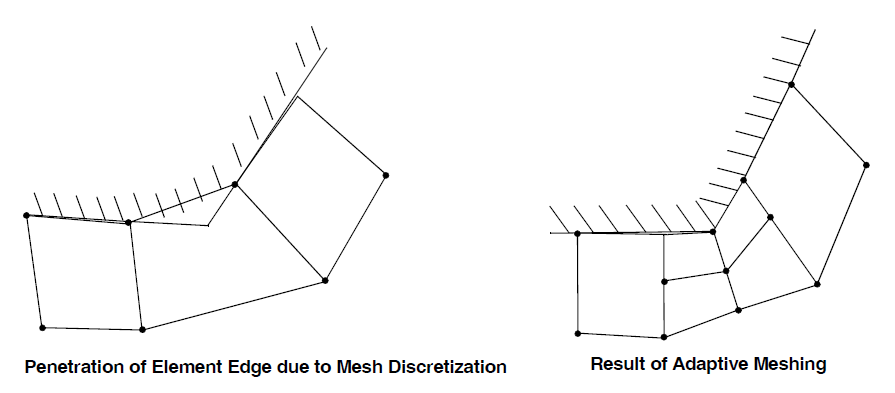
\includegraphics[height=4cm]{img/Adaptive.png}
   \caption{adaptive mesh generation}
 \label{fgr:graft}
\end{figure}



% Hyperelastic Model
\newpage
%\addcontentsline{toc}{section}{\protect\numberline{}{Hyperelastic Materials Modeling}}
%\addtocontents{toc}{\vspace{.5\baselineskip}}
\markright{Hyperelastic Matieral Models}
\section{Hyperelastic materials}
Hyperelastiy is a special case of the classical elasticity brought to extreme conditions. At large strains they behave and in a nonlinear fashion in contrast to the linear stress-strain relation of the small strain elastic behavior. 
Other characteristics include the incompressibility which has direct consequences on the FEM it gives rise to volumetric locking which will be detailed in section 4.2. 
This kind of behavior is usually found in polymer characterized with a cross-linked network

\begin{figure}[h]
\centering
  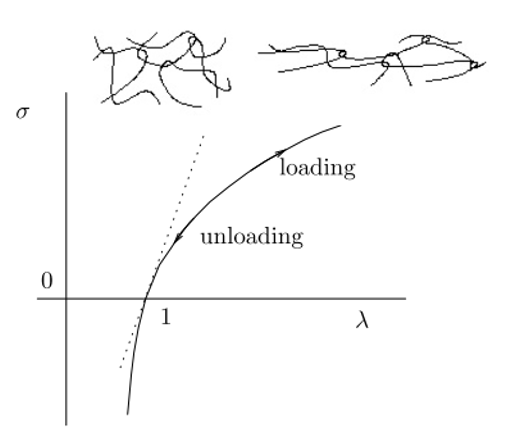
\includegraphics[height=5cm]{img/strainstress.PNG}
   \caption{Non-linear strain-stress curve with above a representation of a compressed an stretched polymer network.}
 \label{fgr:graft}
\end{figure}

The most outstanding property of elastomers is their ability
to undergo large deformations under relatively small stresses and
to retain initial configuration without considerable permanent
deformation after stress removal. This behavior is mostly governed
by changes of network entropy as the orientation of chains alters
with deformation. These basic features can be well described by statistical mechanics as done by Treolar. However, due to the development of computational mechanics and finite element analysis the invariant-based continuum mechanics theory is used to predict rubber elasticity.
\subsection{Constitutive Modeling}
Elastomers exhibit a complicated nonlinear behavior including
hysteresis, viscoelasticity and stress softening phenomenon. The
latter case called Mullins effect, occurs in first cycles of loading. Hysteresis and
viscoelastic behavior take place due to deviation from static
deformation, in which the effects of time and deformation rate
must be taken into account. In the case of static
deformations, rubbers exhibit hyperelastic behavior; Thus, a strain
energy density function, W, can be attributed.
Stress-strain behavior cannot be described by simple hookean law but need something more complex in this case a strain energy density function W. It represents the work that must be done on unit volume of the material in the reference (unstrained) state to deform it to the current configuration. Strictly, W is the Helmholtz free energy in an isothermal process.
For isotropic materials (e.g., rubbers), strain energy function
(SEF) can be represented in terms of right (or left) Cauchy-Green
tensor \textbf{C} (or \textbf{B}) invariants ($I_1, I_2, I_3$) or eigen values of deformation
gradient tensor F, called principal stretches ($\lambda_1, \lambda_2, \lambda_3$). i.e.,
\begin{equation}
W=W(I_1, I_2, I_3)\\
\end{equation}
Where
\begin{align*}
I_1&=\textrm{tr}(\textnormal{\textbf{C}})=\lambda_1^2+\lambda_2^2+\lambda_3^2&\\
I_2&=\frac{1}{2}\left[I^2_1-(\textnormal{\textbf{C}}^2)\right]=\lambda_1^2\lambda_2^2+\lambda_2^2\lambda_3^2+\lambda_1^2\lambda_3^2&\\
I_3&=\textrm{det}(\textnormal{\textbf{C}})=\lambda_1^2\lambda_2^2\lambda_3^2&
\end{align*}
tr and det demonstrate trace and determinant of a tensor. The form
of strain energy density function depends on symmetry, thermodynamic,
energetic and entropic considerations. For example, in the
case of rubber-like materials, due to the negligible compressibility
under conventional pressures, incompressibility assumption is
often used ($I_3 = 1$).

\begin{equation}
W_R=\sum_{i,j=0}^{\infty} C_{ij}(I_1-3)^i(I_2-3)^j
\end{equation}

If a compressibility term is added it gives the expression of the generalized Rivlin model, a general
If only the first term is maintained one obtains the Neo-Hookean model.

\begin{equation}
W_{NH}= C_{10}(I_1-3)
\end{equation}

While if keeping the second term gives rise to the Mooney-Rivlin model.
\begin{equation}
W_{MR}= C_{10}(I_1-3)+C_{01}(I_2-3)
\end{equation}
Working with the framework of the generalized Rivlin model, also called polynomial hyperelastic model, other scientists have come up withhigher order models  to better predict the deviation from the neo-Hooken behavior at large stretches. Among them are: Yeoh, Gent, Arruda \& Boyce.
Another model of high value is the Ogden model, based on a stretch continuum mechanics treatment.
\begin{equation}
W_{O}= \sum_n \frac{\mu_n}{\alpha_n}(\lambda_1^{\alpha_n}+\lambda_2^{\alpha_n}+\lambda_3^{\alpha_n}-3)
\end{equation}
where $\mu_n$ and $\alpha_n$ are real constants.
One approach consists in dividing the strain energy function into deviatoric strain and hydrostatic strain.
\begin{equation}
W=W_D(I_2,I_2)+W_H(J)
\end{equation}

\subsection{Software implementation}
Material curve fitting allows you to derive coefficients from experimental data that
you provide for your material.
• With this capability, you compare experimental data versus program-calculated data
for different nonlinear models and determine the best material model to use.
• ANSYS provides curve-fitting, based on experimental data, for all of the available
hyperelastic models. Any of the hyperelasticity models in ANSYS can be used.
ANSYS implements both a linear and a nonlinear least-squares fit procedures for fitting the data•The common test types include:
 –Uniaxial test –Equi/biaxialtest –Shear test (planar test) –Volumetric tes
 
 Depending on the model you choose, hyperelastic curve fitting can be a linear or a nonlinear regression process. In both cases, the initial coefficients you supply will determine how accurate and efficient your curve fit will be. The initial values of the coefficients generally come from experience, and also from studying the function that defines the model you are attempting to compare/fit your data to. For most hyperelastic models, 1 or -1 is a good starting point. However, coefficient values can vary greatly depending on the model chosen. The Gent model, for instance, provides good fit with initial coefficient values as high as 1000. 
 
 Your error norms can be either normalized or non-normalized. Normalized error norms (the default regression option) generally give better results than the non-normalized error norms, since normalized error gives equal weight to all of your data points.

The solution control parameters of a nonlinear regression include:

    Number of iterations

    Residual tolerance

    Coefficient change tolerance

The solution stops when both the residual tolerance and the coefficient change tolerance of your error norm are met, or if the number of iterations criteria is met. When you use nonlinear regression, you must initialize your coefficients. 

The two factors you consider in determining results acceptability are visual fit and the error norm/residual values. When you plot the curve, the error norm/residual values are printed in the curve-fitting GUI window. Error norm values help you determine the quality of curve fitting and whether to accept the results, but are not always the best indicator of a valid curve fit. Plotting the curves and visually assessing the result is usually the best indication.
\subsubsection{Curve Fitting Problem}
Curve Fitting aims to fit one or more parameters of a model equation $\sigma ( \lambda$, Parameters) in such a way that a given curve $\sigma_M(\lambda)$ is approximated as closely as possible. In this
study, the stress-strain curve for simple shear and the combined stress-stretch curve for
tension and compression have to be approximated. The stress-stretch curve in tension
and compression will be used to explain the regression analysis process. The process for
simple shear is analogous.
Ideally, the fitted model equation resulting from regression analysis should yield the
same stress values as the measured curve.
\begin{equation}
\sigma(\lambda, \textnormal{Parameters})=\sigma_M(\lambda)
\end{equation}

Where $\sigma ( \lambda$, Parameters) is the model function, which depends on stretch and parameters,
and $\sigma_M(\lambda)$ denotes the measured stress-stretch curve.
The model equation for compression and tension is
\begin{equation}
\sigma=f(\lambda, C_{10}, C_{01}, C_{20}, C_{02}, C_{11})
\end{equation}

The parameters (material constants) $C_{ij}$ are considered constant and have to be determined
through regression analysis. Furthermore, in the compression/tension model
equation, they only appear linearly. As the number of data pairs within the measured
stress-stretch curve greatly exceeds the number of parameters within the model equation,
the problem definition is to solve an overdetermined system of linear equations
(Hartmann 2001) in such a way that a satisfactory goodness of fit is achieved.

\subsubsection{Regression analysis}
In general, the overdetermined system of linear equations from subsection 2.2 cannot be
solved. In order to overcome this problem, regression analysis can be applied. A set of
parameters, which yields to a curve that is as close to the measured curve as possible, has
to be determined. For a satisfactory curve fit, the difference between the stress values of
the measured curve and the model equation has to be small for a wide rage of stretches.
The least squares method uses the sum of the difference of the ordinates of two stress
values as an error criterion (Papula 2008, p. 691), which has to be minimized:
\begin{equation}
\epsilon_{ls}=\sum^n_{i=1}\left(\sigma_M(\lambda_i)-\sigma(\lambda_i, C_{10}, C_{01}, C_{20}, C_{02}, C_{11})\right)^2 
\end{equation}
Where $\epsilon_{ls}$: Least square error, $i$: Number of measured data pairs, $\lambda_i$: Measured stretch value, $\sigma_M(\lambda_i$: Measured stress at $\lambda_i$, $\sigma(\lambda_i, C_{10}, C_{01}, C_{20}, C_{02}, C_{11})$: Computed stress value of the model function at $\lambda_i$.
In ANSYS1, the above equation is called “unnormalized least squares fit” ANSYS Inc. (August
2002).
Since it is biased towards higher stress values, a weighted error criterion is
more useful in many cases. Equation 32 accounts equally for every stress value and is
called “normalized least square fit” ANSYS Inc. (August 2002).
\begin{equation}
\epsilon_{norm}=\sum^n_{i=1}\left(1- \frac{\sigma(\lambda_i, C_{10}, C_{01}, C_{20}, C_{02}, C_{11})}{\sigma_M(\lambda_i)}\right)^2 
\end{equation}

Note that Equation 32 would lead to a division by zero if $\sigma_M(\lambda_i)=0$. For this case
an exception has to be added. 
The software ANSYS offers a curve fitting module for hyperelastic material models.2
However, despite supporting higher order constitutive equations for input of material
constants, not all supported material models can be fitted up to these orders. Hence,
the Equations 20 and 28 and both error criteria3 were implemented in a Scilab4 script in
order to be able to fit higher order constitutive equations. The minimization algorithm
used in Scilab is Nelder-Mead (Nelder \& Mead 1965).

Curve fitting algorithm
The material constants are determined by a least-squares procedure for a given set of experimental data, which minimizes the relative error, solution.
The Mooney, Polynomial, Yeoh strain energy potentials are linear in terms of the constants. Therefore a linear least-square fit procedure is used.
The Ogden, Arruda-Boyce , Gent strain energy potentials are nonlinear in terms of the constants. A nonlinear least-squares fitting procedure is neede. We use Marquard-Levenberg algorithm.

\subsection{Numerical issues}
\subsubsection{Incompressibility and Volumetric Locking}
The Poisson ratio ($\nu$) of an isotropic material is usually defined as the ratio, taken with the
opposite sign, between its lateral and longitudinal strains under the action of longitudinal
stresses. 
Some materials exhibit isochoric deformation. This means that the volume of the body stays constant and thus $\nu = 0.5$. If displacement based low-order continuum elements are used this situation cannot be properly simulated. Such elements behave excessively stiff and are said to undergo volumetric locking. Fully integrated and linear brick elements suffer from this issue.  The trivial solution is to use higher order elements. As such, these have higher degrees of freedom so even if incompressible, the strain can still be variable in the element. Higher order elements solve the problem, but are computationally costly. A cheaper solution is using under integrated elements. As only one integration point is available in the center, strain is constant but locking does not occur, however higher mesh density will be necessary.  Another solution is to separate volumetric strain $\epsilon_v$ from deviatoric strain $\epsilon_d$. THe former are integrated in the center and the latter using the full
Although they are considered incompressible they are actually only nearly incompressible. This aspect can be integrated into FEM for complex deformation to help avoid numerical problems that can arise due to incompressible formulations. 
The term $\sum^N_{k=1}\frac{1}{d_k}(J-1)^{2k}$ where $d_k$ is the incompressibility parameter
\subsubsection{Mixed formulation}
\subsubsection{Reduced integration}

\subsubsection{Shear locking}
Full and reduced integration 
\paragraph{Mixed Formulation}
\subsubsection{Hourglassing}



% Contact Model
\newpage
%\addcontentsline{toc}{section}{\protect\numberline{}{Contact Modeling}}
%\addtocontents{toc}{\vspace{.5\baselineskip}}
\markright{Contact Modeling}
\section{Contact modeling}
The objective of contact analysis is to answer the following questions:
(a) whether two or more bodies are in contact, (b) if they are, where the location
or region of contact is, (c) how much contact force or pressure occurs in the contact
interface, and (d) if there is a relative motion after contact in the interface.

Contact is categorized as boundary nonlinearity, in contrast to both geometric
nonlinearity, which emerges from finite deformation problems, and material
nonlinearity, which is a product of nonlinear constitutive relations. The nonlinearity
of contact can be explained in two aspects. Firstly, if two separate bodies come into
contact, the graph of the contact force vs. displacement looks like a cliff because the
contact force stays at zero when two bodies are separate and increases vertically
after the bodies come into contact. In such a case, a functional relationship is not
available because there is no one-to-one relationship between contact force and
displacement. A similar phenomenon happens in the tangential direction under
friction where two bodies are stuck together until the tangential force reaches a
threshold, after which continuous sliding occurs without further increasing the
tangential force. Such an abrupt change in contact force and slip makes the problem
highly nonlinear. Secondly, in order to be a well-posed problem in mechanics,
either displacement (kinematics) or force (kinetics), but not both, must be given for
every material point. Then, the finite element equation solves for unknown information
with given information. On the displacement boundary, for example, if
displacement is given, reaction force should be calculated. On the other hand, on
the traction boundary, if the applied force is given, the corresponding displacement
is to be calculated. Note that these two boundaries are clearly identified in the
problem definition stage. In the case of contact, however, both displacement and
contact force are unknown, except for very limited cases; that is, the contact
boundary is a part of the solution. The user can only identify a candidate of contact
boundary before solving the problem. Therefore, the finite element analysis procedure
must find (a) whether a material point in the boundary of a body is in contact
with the other body, and if it is in contact, (b) the corresponding contact force must
be calculated. Since the contact force at a material point can affect the deformation
of neighboring points, this process needs to be repeated until finding right states for
all points that are possible in contact. Because of this procedural nature, contact
nonlinearity is often addressed algorithmically (Fig. 5.1).
Frictional, frictionless 
\subsection{Contact Formulations}
Surface description, tolerances, separation, adaptive meshing
\paragraph{Surface description}
\paragraph{Tolerances}
\paragraph{Separation}
\paragraph{Adaptive meshing}
\subsection{Governing equations}


\subsection{Discretization}
Discretization of the contact area into elementary units responsible
for the contact stress transmission from one contacting surface to
another.
Node-to-node discretization
Node-to-segment discretization
Segment-to-segment discretization
Mortar and Nitsche discretizations
Contact domain method for discretization


\subsubsection{Smoothing}
Scheme of two non-matching meshes
Smoothing of the master surface
Contact detection
Contact element construction (edge contact element)
Constructed smoothed contact elements

\subsubsection{Solution}
Boundary value problem with constraints

\subsection{Optimization methods}
Smoothing algorithm 
\subsubsection{Penalty}
\subsubsection{Lagrange multipliers}
\subsubsection{Augmented Lagrangian}





% Results
\newpage
%\addcontentsline{toc}{section}{\protect\numberline{}{Results}}
%\addtocontents{toc}{\vspace{.5\baselineskip}}
%\markright{Results}
\newpage
\part{Results and Discussion}
This part is organized as follows. First, in the 7th chapter a preliminary analysis is done to characterize the problem and plan the experiments and simulations. Then, in the 8th chapter, the finite element model construction and the simulations are exposed. In the 9th chapter the experiments coupled with the design of experiments methodology are illustrated. Finally, this part is concluded with the discussion in chapter 10 where the main results are put in perspective and compared between simulations and experiments.

\section{Preliminary analysis}

In this first results and discussion chapter I will start by approach by first giving the general context and background of PFS manufacturing in order to understand its components, its function and how they are interlinked. Then, I further investigate the Plunger assembly step and its characterization methods. After, I deconstruct the problem to understand the physics and dividing it into underlying phenomena. Finally, I identify what factors might have an influence on the stages of the assembly and based on the I list the needed experiments and simulations to test the hypothesis and quantify the impact on the process outcome quality (see Figure \ref{fgr:cat}.

\begin{figure}[h!]	
	\centering
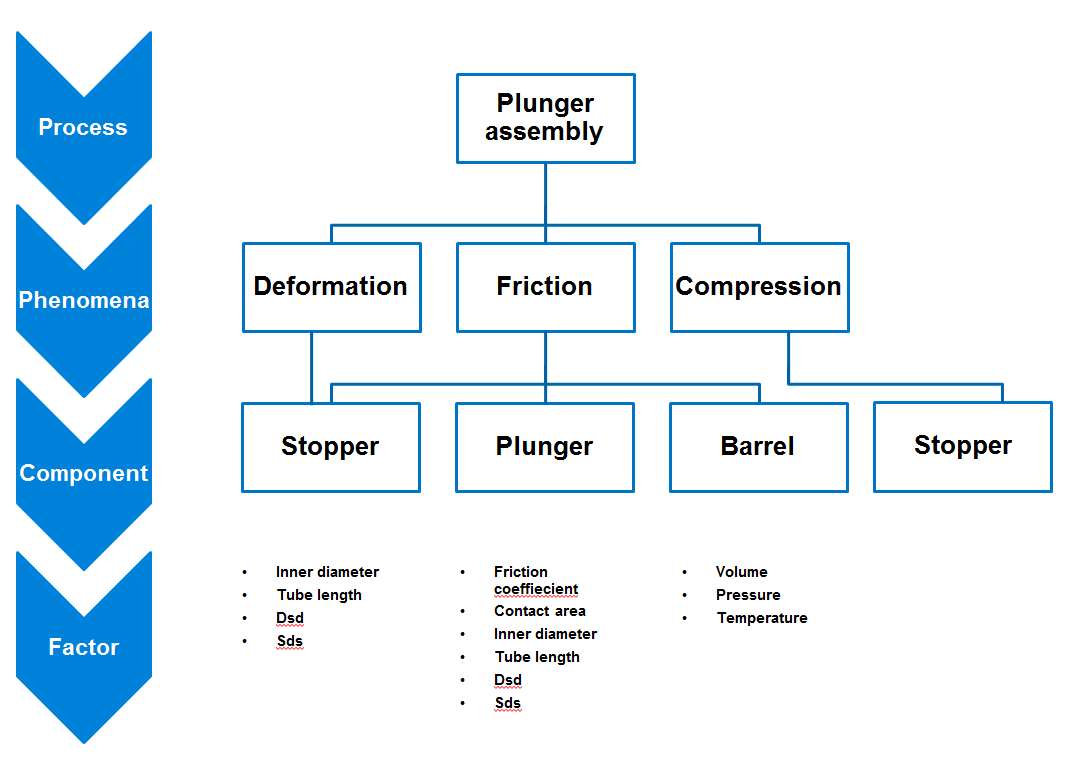
\includegraphics[height=9cm]{img/category.PNG}
   \caption{PR Assembly Step Break-down}
 \label{fgr:cat}
\end{figure}

\newpage
\subsection{Prefilled Syringe manufacturing}

\subsubsection{Components}
The Prefilled Syringe main components are a glass barrel, a rubber stopper, a polymeric tip cap, the liquid medium, a  polymer plunger and a extended finger flange (see Figure \ref{fgr:PFS}). 

\begin{figure}[h]	
	\centering
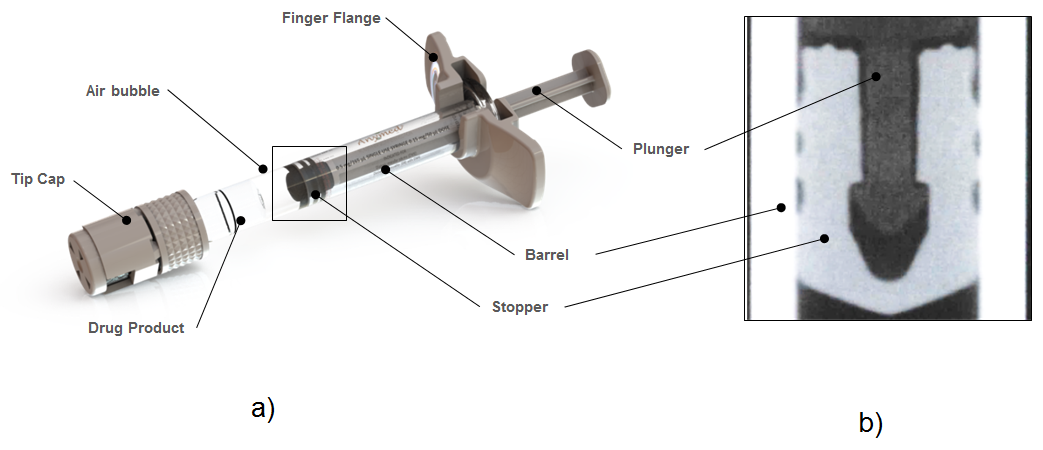
\includegraphics[height=6cm]{img/PFS.PNG}
   \caption{Representation of a) Prefilled  Syringe with described components and b) a Computer Tomography Scan of the Stopper - Plunger snap-fit geometry highlighted in part a).}
 \label{fgr:PFS}
\end{figure}

All of the components can vary depending in design on the requirements but each has a specific role for the drug delivery. A central quality attribute a PFS has to assure is the maintenance of the sterility of the drug product during the whole manufacturing process until it arrives to its end user, the patient. The stopper plays a central role as it provides the barrier separating the medium from the outside. Silicon oil is the invisible component that makes the gears turn as it ensures the isolation, while ensuring the right injection force necessary to deliver the drug. The plunger is the handle, the trigger that enables the administration by pushing downwards the stopper. As described in the problem statement this specific model a snap-fit mechanisms is used to keep the two components together. 

\begin{table}[h]
\def\arraystretch{1.4}
\caption{PFS Components, material composition and fucntion}
	\begin{tabular}{p{2.6cm} p{3.7cm}p{9cm}}
	Components & Material & Function \\
    \hline
Syringe Barrel  & Glass         & Medium container \\
Silicon oil     & Oil           & Lubricant and sealant \\
Tip Cap         & Polymers and rubber & Connection channel for the drug product to the needle\\
Drug Product    & Liquid suspension & Cure the disease\\
Air bubble      & Ambient air   & Separation between medium and stopper \\  
Stopper         & Rubber        & Sealant and drug delivery\\  
Plunger         & Polypropylene & Push or pull the stopper\\
Finger Flange & Polymer & Handle and counter force to the patient for delivery\\
\hline
	\end{tabular}
\end{table}
\newpage
\subsubsection{Manufacturing process}

The manufacturing of a PFS can take place in different locations depending on the production capacity. Although it has few components, strict safety regulation demands for extra requirements during the production. Each step can happen in a different site. 
The stages of manufacturing are depicted in the following figure \ref{fgr:manu}.

\begin{figure}[h]	
	\centering
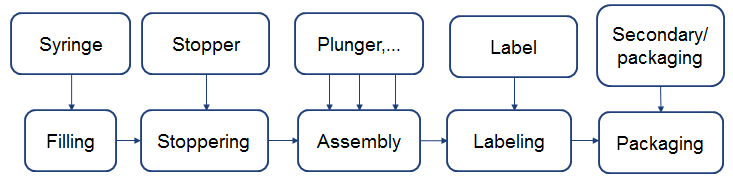
\includegraphics[height=4cm]{img/pfs_manu.PNG}
   \caption{Flowchart of the PFS manufacturing process.}
 \label{fgr:manu}
\end{figure}

\subparagraph{Syringe production}
It is necessary to coat the inner surfaces of the syringes with a layer of silicone. The silicone is either applied by spraying
silicone oil onto the glass or by coating the glass with a silicone emulsion that is baked onto the glass. A covalent atomic bond results in the barrel and the rest of the silicon oil is still freely movable thus less silicon oil is needed do reach a homogeneous distribution compared to spray siliconization[1]. Spray siliconization is applied with static nozzles and movable nozzles, which dive in the barrel providing a more homogeneous distribution. 
\subparagraph{Aseptic filling}
Pharmaceutical manufacturing companies that prefilled syringes may receive the syringes ready-to-use or as bulk syringes. Companies that choose to work with bulk syringes will clean, sterilize and apply silicone at their facilities. Ready-to use syringes are pre-cleaned, pre-sterilized and, if needed, siliconized.
The equipment can be paired with a variety of filling pumps. The types of filling pumps available include a diaphragm pump, rotary peristaltic pump, rotating piston pump and a time/pressure filler. All systems have their advantages and disadvantages.
\subparagraph{Stopper placement}
The goal is to place the stopper near the surface of the solution without touching the liquid. A gap of approximately 4$\pm$2mm is left between the solution and the surface of the plunger. Placement of the plunger closer to the solution risks the solution escaping around the edges of the plunger and leaving droplets of liquid between the ribs of the stopper, they are seated by one of two mechanisms. Vent-tube stoppering (see Figure \ref{fgr:stoppering} below) collects the plunger in stainless steel tubes that compress the plungers and a plunger insertion rod pushes the plunger into the syringe barrel. Compressing the plunger before placement allows air to escape around the plunger so that it will remain in place when it expands to fit into the barrel. 

\begin{figure}[h]	
	\centering
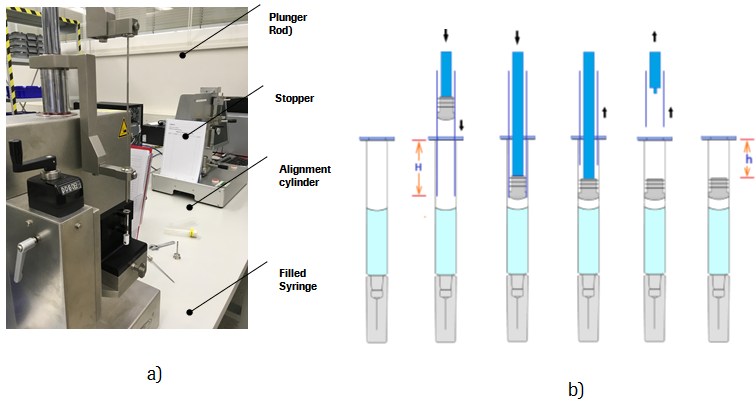
\includegraphics[height=6cm]{img/stoppering.PNG}
   \caption{a) Picture of the stoppering machine (B\&S) and b) scheme of the stoppering process.}
 \label{fgr:stoppering}
\end{figure}

%Vacuum stoppering operates with negative pressure to place the plungers. The stopper slides in the syringe barrel and stack up a silicon oil ring which has an influence to $d_{oil}$. Plungers are collected into a cylinder and the cylinder makes contact with the top of the syringe. A vacuum is pulled through the cylinder to remove air and the plunger is vacuumed out of the tube and into place in the barrel of the syringe. There are some syringes that are only compatible with vacuum plunger placement.

\subparagraph{Plunger assembly}
The plunger does not have to be connected with the stopper, as a matter of fact, designs exist without any plunger pin. However, disconnecting involves risking that the plunger might fall off if the PFS is turned upside down. Another common way of connecting the two is with a screw-in mechanics the assembly machine required thus torque and a mild downward movement.
The most common system is to place cameras. For assembly machine that check the distances, before and the insertion and if there are any gaps.
\begin{figure}[h]	
	\centering
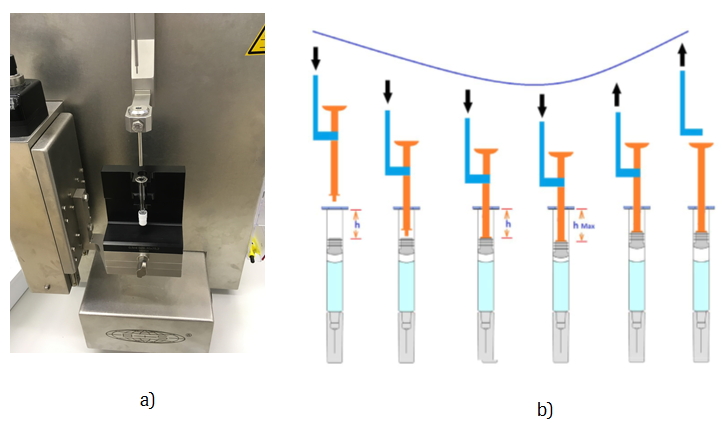
\includegraphics[height=7cm]{img/plungering.PNG}
   \caption{a) Picture of the stoppering machine (B\&S) and b) scheme of the plunger assembly process.}
 \label{fgr:PFS}
\end{figure}

\newpage
\subsection{Plunger assembly characterization}
The main measurement technique is with a tensile machine where the plunger is pushed by a stamp with is connect to a force sensor. Starting from the beginning: the plunger is lowered into the stopper until the plunger pin tip touches the inner walls of the stopper. The plunger starts the insertion by deforming the stopper walls pushing towards the exterior, thus increasing the contact area between the three components. This goes on until the pin is fully inserted into the stopper cavity, ending the first section of the force-displacement curve (see Figure \ref{fgr:force}). At this point the stopper and plunger have gained enough common surface area, allowing it to surmount the break loose force $F_{BL}$ necessary to overcome the static friction between barrel and stopper. This results in a sharp drop in force and a downwards displacement of the stopper. This movement causes the air bubble situated between the stopper and the medium to compress until the pressure is built up enough to compensate the static friction between the plunger and the stopper. This 2nd step is represented by curve in the force-displacement diagram and can also be derived theoretically with Boyle's law, as will be shown later. Once the air pressure is enough the insertion process continues, overcoming the maximum required force until the snap-in, which can be seen as a plateau and than a sharp drop. This gives a measurable parameter: the maximal force $F_{max}$.  Last but not least, if the compression continues the reaches a hard stop, given by the combination of the maximum compression of rubber, air, and liquid incompressibility.

The assembly can be divided in 4 stages as shown in the picture below:


\begin{figure}[h!]	
	\centering
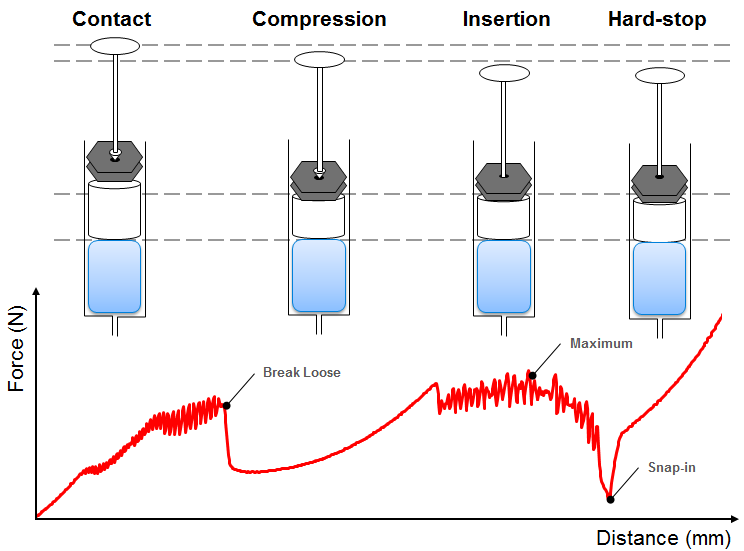
\includegraphics[height=9.5cm]{img/force.PNG}
   \caption{Plunger Assembly Step characterization}
 \label{fgr:force}
\end{figure}


\newpage
\subsection{Physical phenomena}
In order to fully comprehend the process it is necessary to study the single handedly. This next subsection I would like to give more detail on how these single phenomena affects the assembly.
Based on this analysis discuss what experiments are necessary to build the model. 
As seen above all steps have to some degree involved with material deformation, friction between the stopper-plunger and stopper-syringe with addition of air bubble compression in the second step.
The system is mainly friction dominated and thus this defines which component of the system is going to move: the plunger or the stopper.
In the following table the stages are shortly summarized and the involved phenomena.

\begin{table}[h]
\def\arraystretch{1.5}
\caption{Plunger assembly steps.}
	\begin{tabular}{l p{6cm}p{5cm}}
	Phase & Description & Acting Phenomena \\
    \hline
    1. Contact      & Plunger touches the stopper and compresses it & Hyperelastic deformation, Static Friction \\
    2. Compression  & Break loose: air bubble compression and stopper movement   & Dynamic friction, air pressure increase\\
    3. Insertion    & Given the air bubble pressure, the plunger is inserted until snap-in                         & Air pressure, Static friction\\
    4. Hard stop    & Further compression                           & Deformation, air pressure\\
    \hline
	\end{tabular}
\end{table}

\subsubsection{Deformation}
Rubber deformation, in contrast with other plastics and common polymers, is described by hyperelastic strain energy density laws. This is the case because rubber behaves similarly to elastic materials but is nonlinear. As such, there are a number of models which aim to describe the behavior for the different deformation modes of the material.
The stopper is going through different types of deformation during the assembly process. First, in the stoppering a concentric compression is applied in order to fit in the syringe cavity. Then, during the plunger insertion process, the walls are pushed to the side by the plunger pin which makes its way into the tube. Finally, at the snap-in the stopper reaches maximum strain.
\begin{figure}[h!]	
	\centering
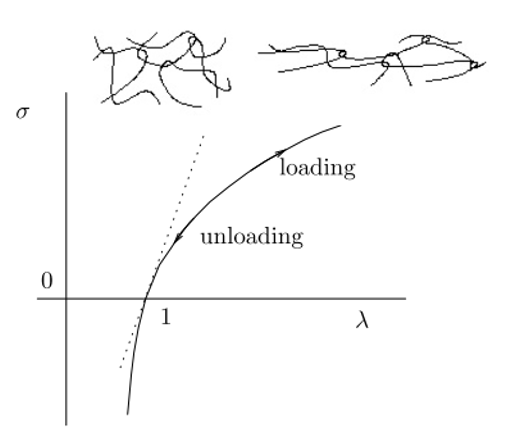
\includegraphics[height=3cm]{img/strainstress.PNG}
   \caption{PR Assembly Step Break-down}
 \label{fgr:PFS}
\end{figure}

\newpage
\subsubsection{Friction}
 There are many factor involved in this and they are represented below
As the picture below illustrates, the Ishikawa diagram
\begin{figure}[h!]	
	\centering
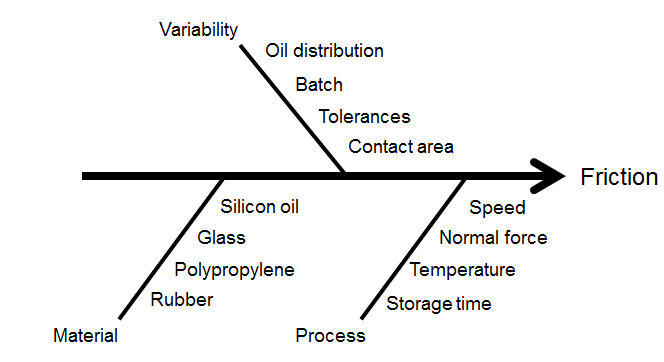
\includegraphics[height=7cm]{img/ishi.PNG}
   \caption{Strain stress curve and ishikawa for mat def}
 \label{fgr:PFS}
\end{figure}

\paragraph{Plastic - Rubber}
This interaction is defined by the materials which are Bromobutly rubber and polypropylene.
The surface is very rough leading to high friction coefficients
\paragraph{Rubber - Glass}
This is special because it is a wetted contact, namely by silicon oil. This is introduced to the system to allow the delivery and to lower the break loose force required. Thus, although relate to other factors such a speed and geometry break loose force is highly dependent on this silicon layer and has been thoroughly studied in the literature.
\begin{equation}
F_{friction}=\frac{\pi \cdot \mu \cdot l_{stopper} \cdot d_b}{d_oil}\cdot v
\end{equation}

\subparagraph*{Break-loose Force} 	The break-loose force is determined through the static friction between stopper and glass barrel respectively silicon oil layer. Is the maximum detected force to overcome the static friction between glass barrel and stopper. It is a special event in its movement  Once the BLF is overcome, the stopper begins to glide.
The break loose force ($F_{BL}$) is defined as the maximum force required to overcome the static friction between the stopper and the glass barrel.
\begin{equation}
F_{BL}=F_{friction}\frac{d_{b} \cdot l_b}{d_{b} \cdot l_{b}}
\end{equation}


\subsubsection{Air bubble compression}
The air bubble is in the system from the beginning and its volume and pressure is dependent on the stopper. 
The size of the bubble is defined by the space between the drug product and the stopper, this distance is called headspace.
This component is central to the plunger insertion as it provides the necessary reaction force to allow for it. However, this will only be the case if it is compressed enough. Unfortunately, the standard stopper placement technique is vent tubing, thus the bubble has air pressure of 1 atmosphere. Consequently, the stopper has to move in order for the bubble to build up enough pressure. The force applied by the air can be derived from Boyle's law. If we approximate the air column to a cylinder.
\begin{eqnarray}
p_1V_1=p_2V_2; p_2=p_1\frac{V_1}{V_2}\\
p_2=p_1\frac{h_1}{h_2}; V=\pi r^2 h\\
F=p_1\pi r^2 \frac{h_1}{h_2} with F=pA
\end{eqnarray}
$h$ is the headspace, p the pressure, V the volume, F the force, A the area, $r$ the radius of the syringe inner diameter. 
\begin{figure}[h!]	
	\centering
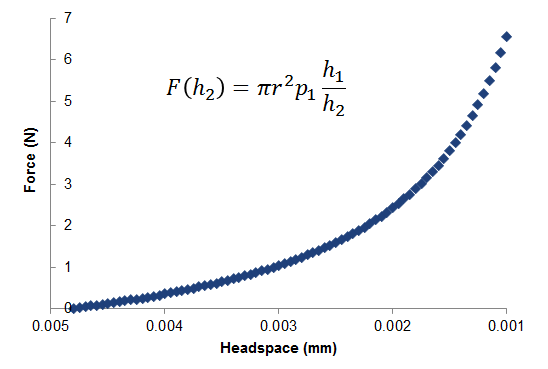
\includegraphics[height=7cm]{img/forceboyle.png}
   \caption{PR Assembly Step Break-down}
 \label{fgr:PFS}
\end{figure}

\newpage
\subsection{Parameter selection}

As described above the main phenomena are air bubble compression, rubber deformation and friction. Of the three aforementioned phenomena there are a number of factors that influence the plunger insertion and they are listed below. These can be studied with experiments and simulation.

\begin{figure}[h!]	
	\centering
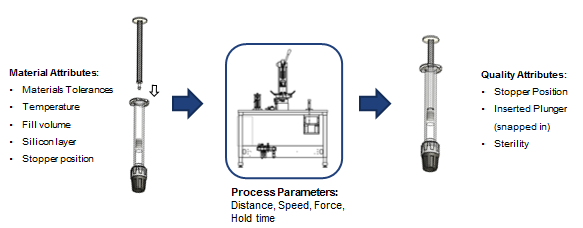
\includegraphics[height=5cm]{img/in_out.PNG}
   \caption{PR Assembly Step Break-down}
 \label{fgr:PFS}
\end{figure}
    
\subparagraph*{In-scope}
 
	Geometry is the most obvious category of parameters that potentially affect the the insertion force. The reason is contact area. Basically, the insertion is enabled by friction or rather a ratio between the plunger/stopper and stopper/glass barrel friction coefficients. Thus, any change in geometry that might increase of lower the contact area between the components I considered, of relevance are thus the plunger pin dimensions, like its length, diameter and cone angle and its negative fit geometry, the stopper inner tube length and diameter. Of importance are also the rip diameter of the stopper and	syringe diameter which determines the stopper compression. A bigger stopper has a bigger surface and the friction depends on the stopper size. Effect through $l_{stopper}$  ,$d_{barell}$
	 Plunger positions affect the variability of the measured syringes regarding to gliding forces[18].
	Environmental factors like temperature and humidity.
    Storage temperature and humidity affects the silicone oil viscosity and material aging. Therefore the material can be changed to slightly different characteristics and the silicon flows out faster. Effect to break loose force $\mu_{oil}$
    
    Friction can be studied as a results of actual forces and can be used as a bulk property in simulations. However, real experiments to determine the friction like roughness of materials or silicon oil inspection is considered out of scope. 
\subparagraph*{Out-of-scope}
Suppliers are NO and GB with different production sites.
Batch variability describes the fluctuations in different batches. 
	Different Materials like other silicone oil, different stoppers or different glasses affect the friction. 
	Vent-tube or vacuum stoppering are different stopper placement processes.  Vent-tube stoppering was applied for all investigated PFS. 
	Parameters of the silicon oil are out of scope thus, technique, oil distribution, its viscosity, interactions and amount
    

\begin{table}[h]
\def\arraystretch{1.5}
\caption{Potential process impact factors}
	\begin{tabular}{p{2 cm} p{2 cm} l l l}
	Category & Component & Factor (symbol) & Specification (unit)& Control  \\
    \hline
    Geometry& Barrel 	& Inner diameter $d_b$& 4.65 $\pm$ 0.1 mm& Caliber\\
    		& Stopper 	& Rib diameter	$d_r$& 5.00 $\pm$ 0.15 mm& CT-Scan\\
			& 			& Inner diameter$d_i$& 1.60 $\pm$ 0.25 mm& CT-Scan\\
            &			& Tube length	$d_l$& 3.20 $\pm$ 0.25 mm& CT-Scan\\
            &			& Position 		$x_s$& 4.87 $\pm$ 1.5 mm& Scale\\
			& Plunger	& Pin diameter	$d_p$& 2.00 $\pm$ 0.07 mm& Scale\\
            &			& Pin length	$x_l$& 5.10 $\pm$ 0.2 mm& Scale\\
    Friction& Silicon oil (stopper, barrel)& Friction coefficient $f_l$&				&	\\
            & (plunger, stopper)& Friction coefficient $f_l$ &				&	\\
  Assembly Parameters&Assembly machine	& Displacement	$x_i$& 6 $\pm$ 4 mm& Computer\\
   					&					&Insertion Speed	$v_i$		& 750 $\pm$ 745 mm/min& Computer\\
                    &					& Hold time	$t_h$	& 2.5 $\pm$ 2.5 s	& Computer\\
  Environment& Ambient Air		& Temperature $T$& 20 $\pm$ 3 $^{\circ}$C & Thermometer\\
   					&					&Humidity	$p$		& 1 $\pm$ 745 atm& hygrometer 
    \end{tabular}
\end{table}

\begin{figure}[h!]	
	\centering
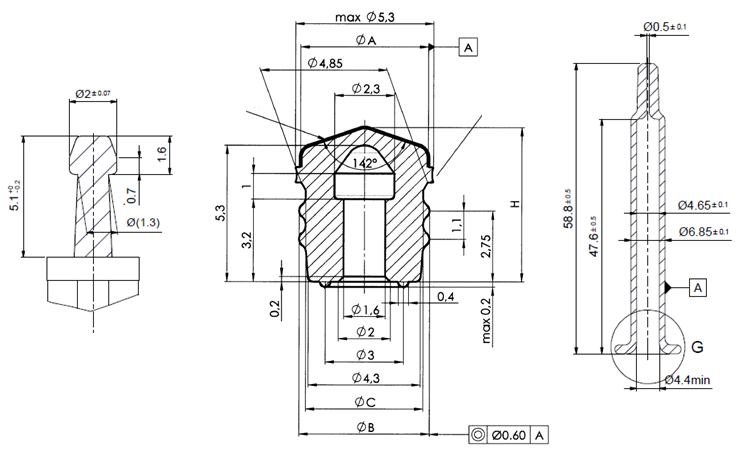
\includegraphics[height=7cm]{img/blueprint.PNG}
   \caption{Blueprints of syringe, stopper and plunger with evidenced components that affect the process}
 \label{fgr:PFS}
\end{figure}

\newpage
\subsection{Testing strategy}
Based on the previous considerations here is a list of experiments where factors have to be discerned and data necessary to be generated.

\begin{figure}[h!]	
	\centering
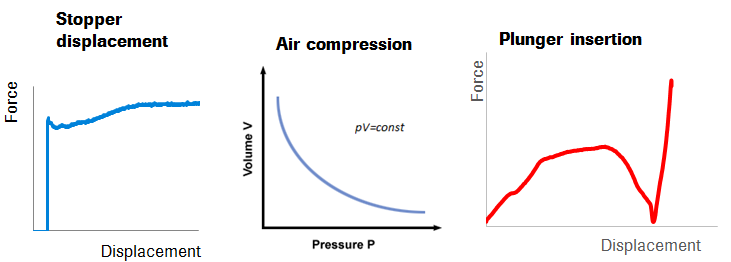
\includegraphics[height=5cm]{img/tests.PNG}
   \caption{Testing strategy}
 \label{fgr:PFS}
\end{figure}

Assume the following are constant: air bubble pressure, water viscosity, silicon oil properties (layer) assembly machine parameters (?), a storage temperature of 25 deg of 3 months



\newpage
\section{Finite element analysis}

\subsection{Finite element model}
Model construction

\subsubsection{Geometry}

CAD, 2D Axisymmetric

\subparagraph*{Spec and variability}
Check real data
\begin{figure}[h!]	
	\centering
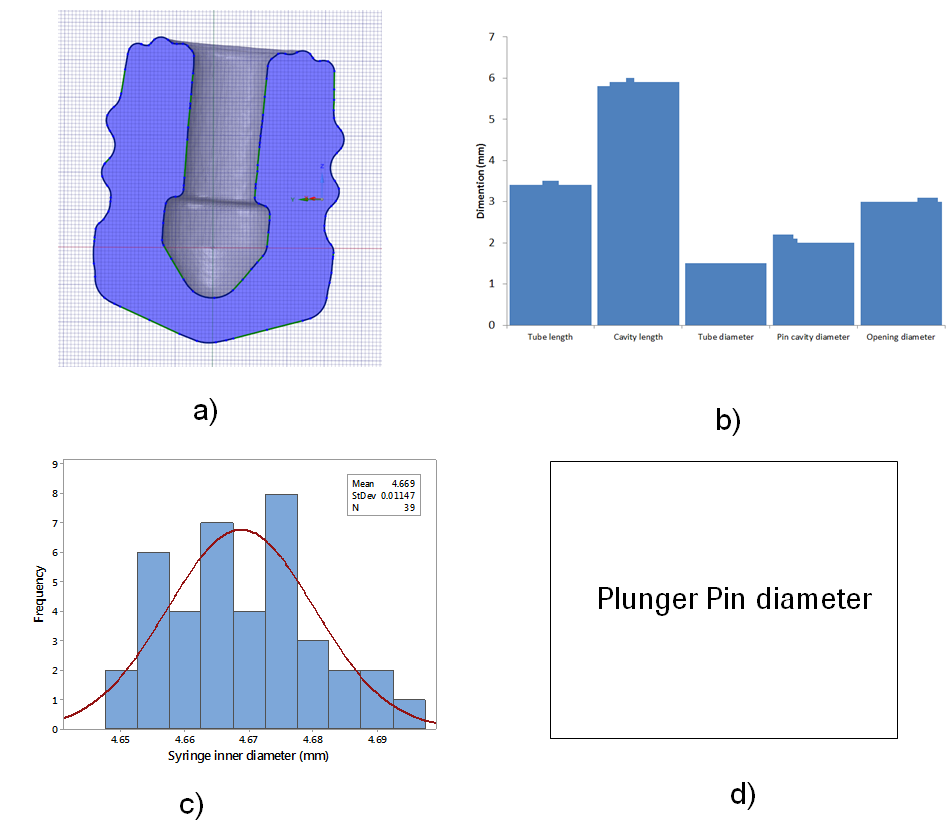
\includegraphics[height=11cm]{img/spec.PNG}
   \caption{Statistics of the measured factors . TO INTEGRATE: scanned stoppers, and their dimensions}
 \label{fgr:PFS}
\end{figure}

\newpage

\subsubsection{Meshing \& Loading}

There are two loading both controlled by displacement and they are first the barrel and then the plunger. The center of reference is the stopper and in order to avoid to simulate the whole stoppering step the stopper position is already there while the syringe is effectively larger thus not touching and not compressing the stopper. The other alternative is to start directly with the original barrel radius however this caused non convergence.

\begin{figure}[h!]	
	\centering
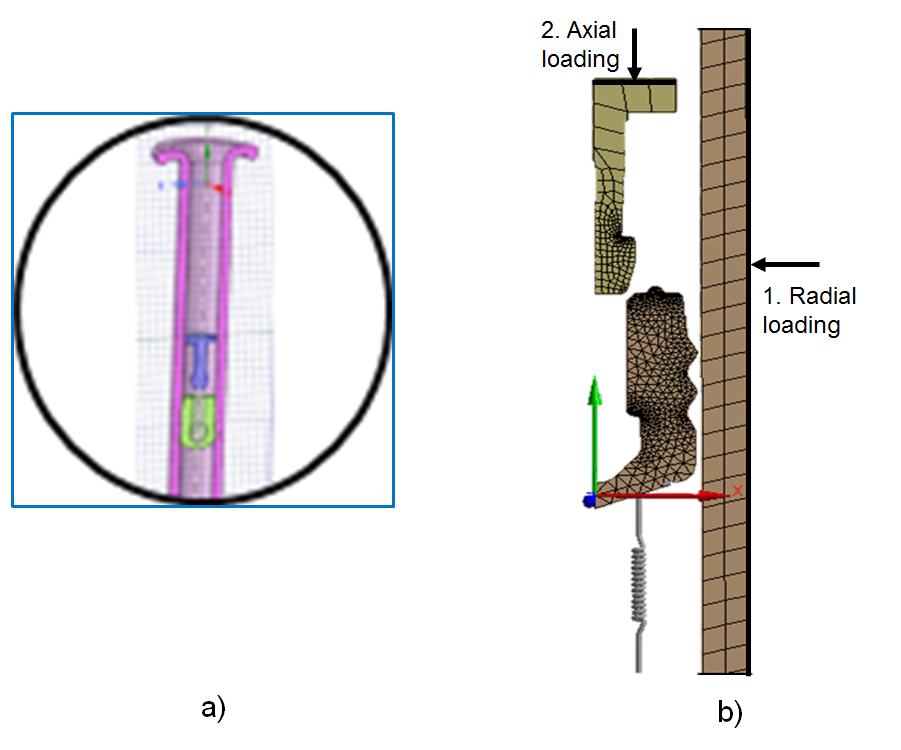
\includegraphics[height=7cm]{img/meshing.PNG}
   \caption{Stopper CAD and scan}
 \label{fgr:PFS}
\end{figure}


\subsubsection{Air bubble}
The air bubble is described by basic thermodynamic laws. FEM doesn't have these and thus there has to be an alternative to describe this and there are some possibilities. Basically, the air bubble pressure depends on its position.
Spring
Elastic material/ material young-s modulus
Challenge spring, nonlinear


\begin{figure}[h!]	
	\centering
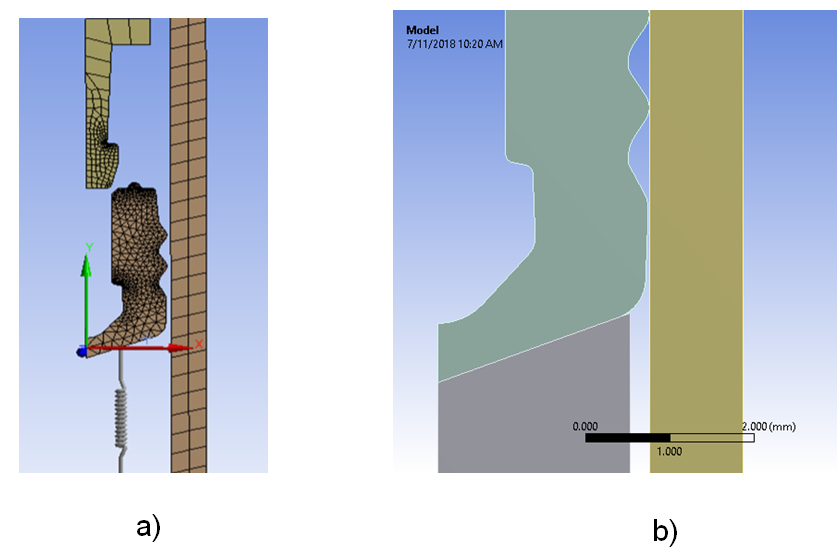
\includegraphics[height=7cm]{img/air.PNG}
   \caption{3D into 2D model}
 \label{fgr:PFS}
\end{figure}

\begin{equation}
\frac{F}{S}=Y\frac{\Delta L}{L}
\end{equation}

\newpage
\subsubsection{Material Data}
Sample, cutting, testing, ASTM, Data fitting

\begin{figure}[h!]	
	\centering
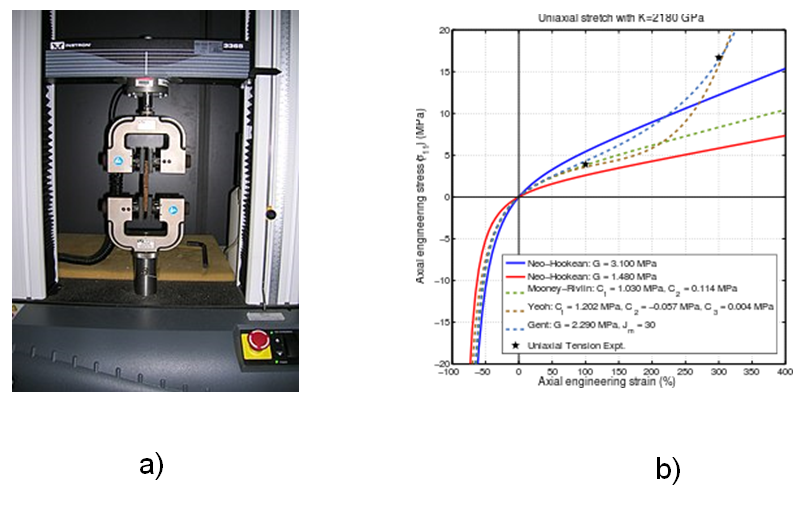
\includegraphics[height=7cm]{img/matdata.PNG}
   \caption{Data and model fitted}
 \label{fgr:PFS}
\end{figure}
Neo Hookean Model / Mooney Rivlin

\newpage
\subsection{Convergence}
Given the nature of the problem the main tools are contact and numerical
\subsubsection{Contact definition}
The tricky part is the friction coefficient ratio.

\subparagraph*{Barrel - Stopper}
This resulted in the less problematic given the right loading approach. The Lagrange is the right tool as it is a classical asymmetric rigid - flexible type of contact. Lagrange delivers thus on the zero penetration condition. Given the smooth compression of the stopper 

\subparagraph*{Stopper - Plunger}
This contact was the most problematic as it caused numerous element distrotions. Penalty method was the way to go in terms of helping the resolution of the problem by imposing less strict boundary conditions with the stiffness coeff. 


\subsubsection{Numerical methods}
Unsymmetric newton raphson explicit, implicit 

\subsubsection{Instability state}
Snap-fit

\subsubsection{Adaptive remeshing}

\newpage
\subsection{Calibration \& Validation}
Static simulation: main tools easier but has limitations: it is not dynamic.

\subsubsection{Stopper compression}
\begin{figure}[h!]	
	\centering
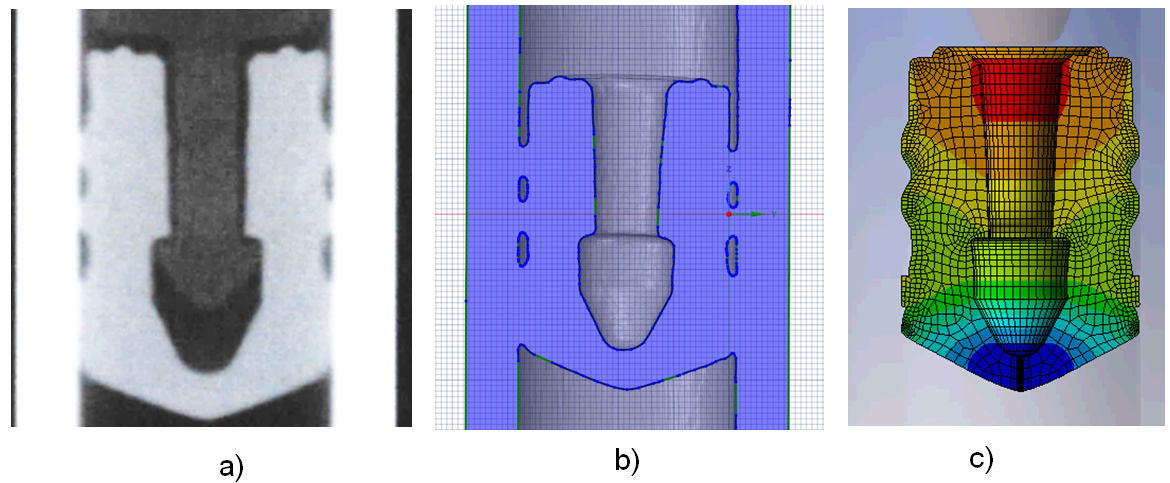
\includegraphics[height=7cm]{img/valicross.PNG}
   \caption{Stopper CT Scan and Simulation}
 \label{fgr:PFS}
\end{figure}

\newpage
\subsubsection{Plunger insertion}

\subparagraph{Frictionless}
Yadeyadeyada
\begin{figure}[h!]	
	\centering
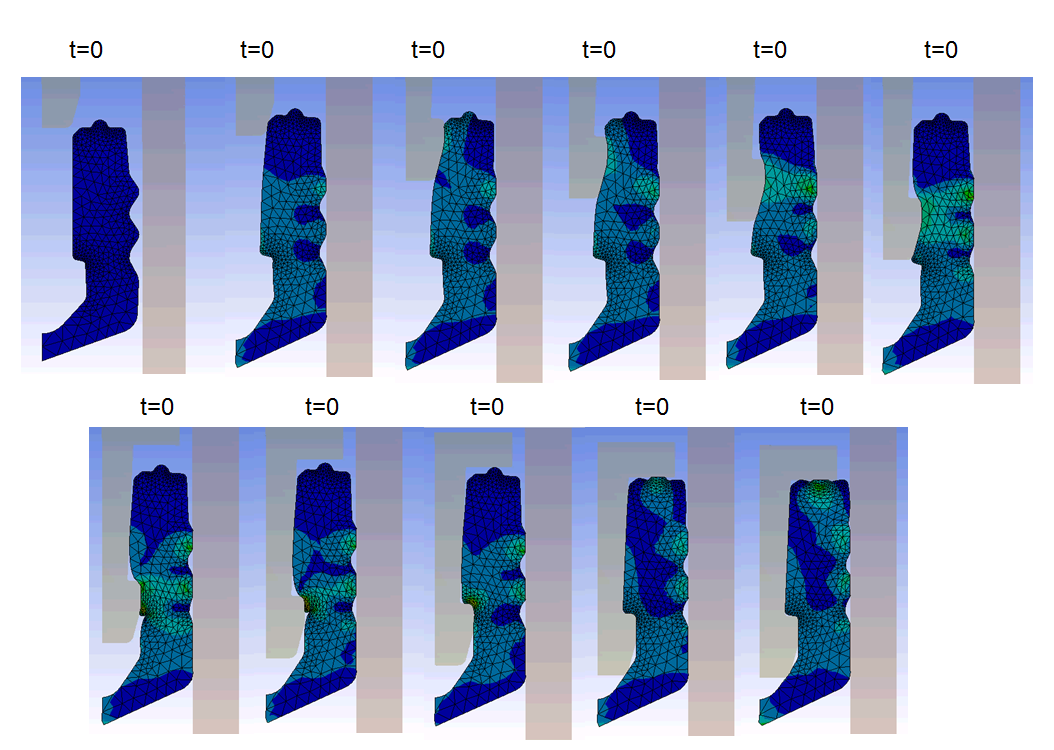
\includegraphics[height=11cm]{img/fricless.PNG}
   \caption{Frictionless plunger insertion sequence}
 \label{fgr:PFS}
\end{figure}

Insertion without problems but yields incorrect results.
\newpage
\subparagraph{Frictional}
Yadeyadeyada

\begin{figure}[h]	
	\centering
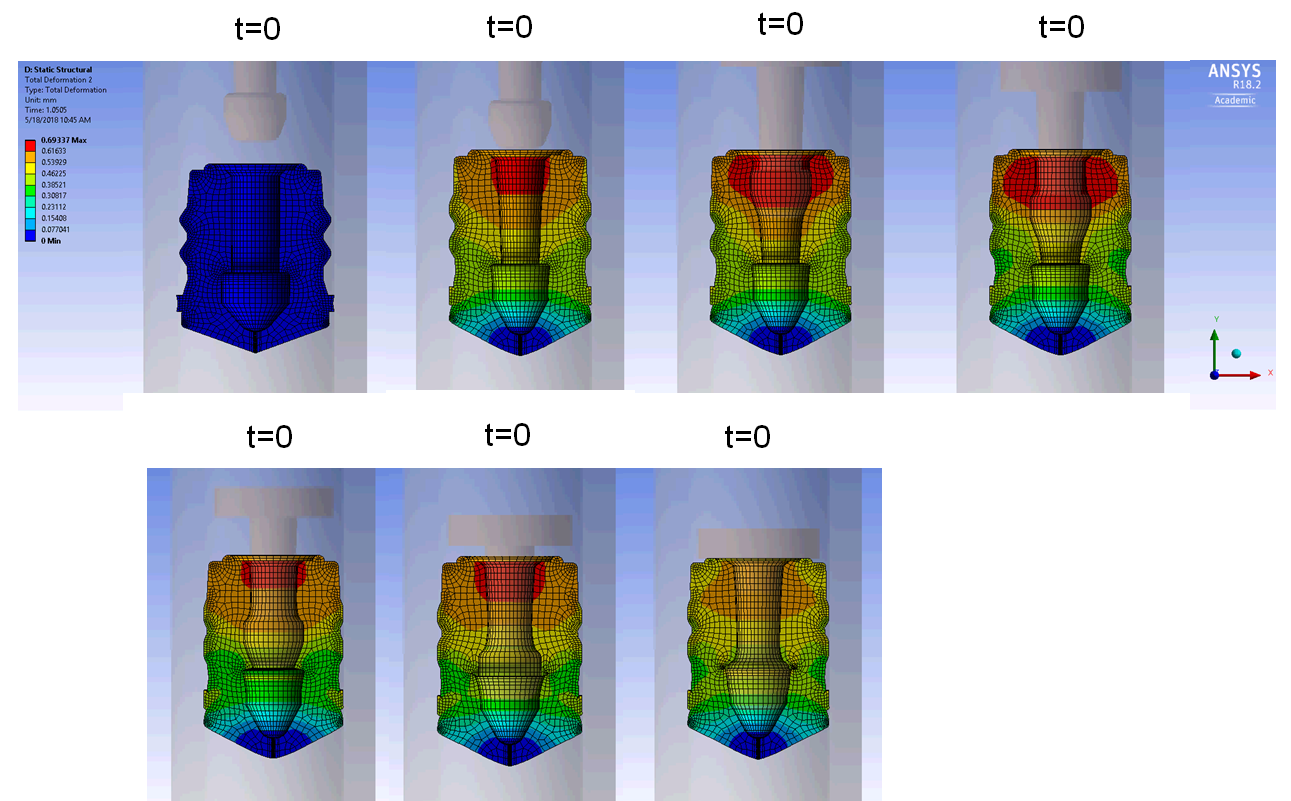
\includegraphics[height=10cm]{img/fric.PNG}
   \caption{Friction plunger insertion sequence}
 \label{fgr:PFS}
\end{figure}

 A singularity forms at the snap-in
 
\newpage
\subsubsection{Stopper movement}
Yadeyadeyada

\begin{figure}[h!]	
	\centering
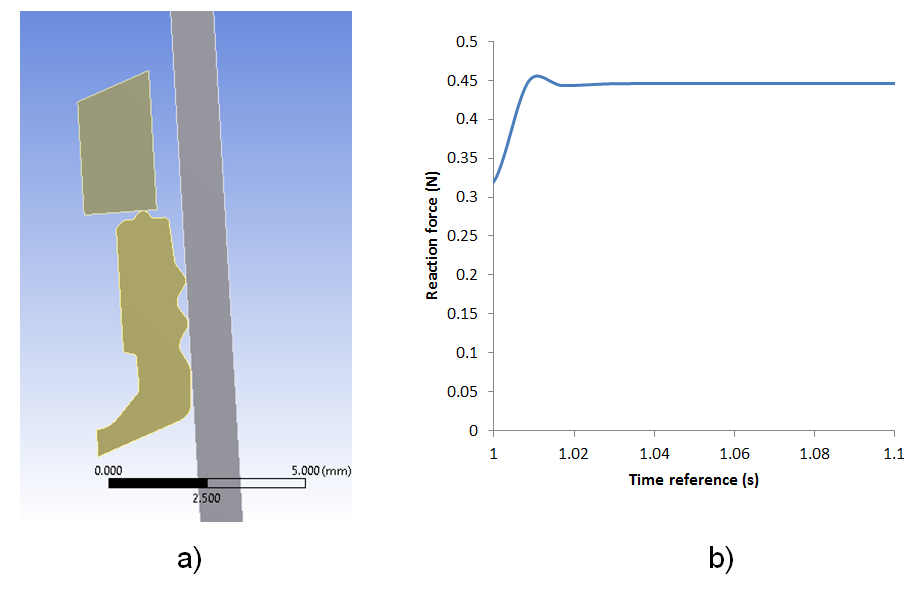
\includegraphics[height=9cm]{img/dyna.png}
   \caption{Simulation of stopper movement for break loose force and dynamic friction.}
 \label{fgr:PFS}
\end{figure}


\subsubsection{Model prediction accuracy}
Slow is OK, fast not OK


\newpage
\subsection{Sensitivity analysis}
Given the problematic snap-in, the focus was laid upon the maximum force and used as parameter for the sensitivity analysis. This is measured by the reaction force of the plunger displacement
\subsubsection{Geometry}
\subparagraph*{Barrel inner diameter}
\subparagraph*{Plunger pin diameter}
\subsubsection{Friction coefficients}

\begin{figure}[h!]	
	\centering
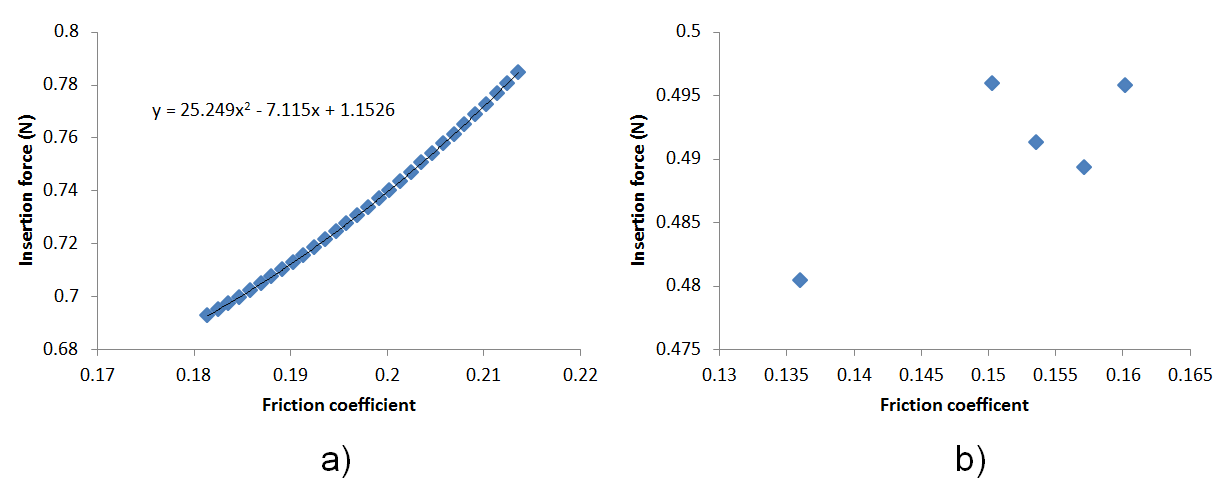
\includegraphics[height=6.5cm]{img/sens.PNG}
   \caption{Friction coeffs sensitivity analysis}
 \label{fgr:PFS}
\end{figure}


\newpage
\subsection{3D Model}
Challenges for meshing




\newpage
\section{Experimental analysis}
\subsection{Set-up}
Lay out
\begin{figure}[h!]	
	\centering
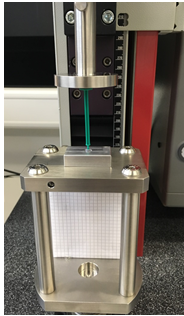
\includegraphics[height=5cm]{img/setup.PNG}
   \caption{PR Assembly Step Break-down}
 \label{fgr:PFS}
\end{figure}

\subsubsection{Materials}
\subsubsection{Methods}

 
\subsection{Design of experiments}
\subparagraph*{Screening}
Goes together
\begin{figure}[h!]	
	\centering
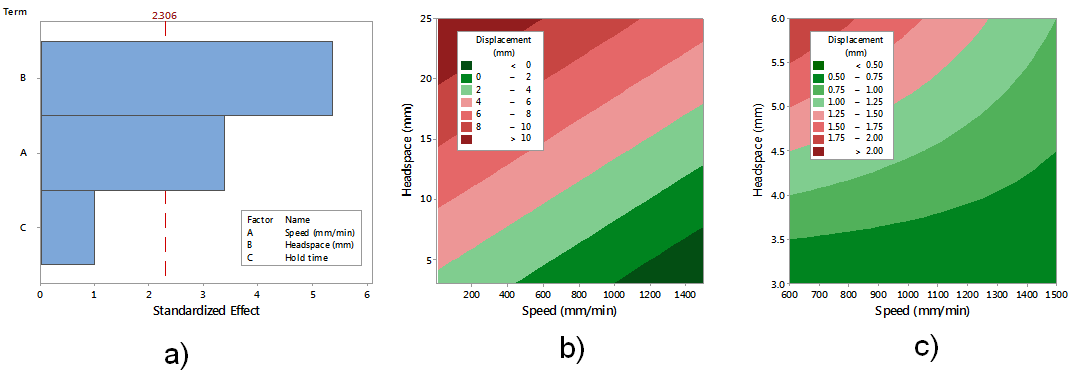
\includegraphics[height=5cm]{img/screen.PNG}
   \caption{PR Assembly Step Break-down}
 \label{fgr:PFS}
\end{figure} 

\subparagraph*{Factor selection}
Screening

 
\subparagraph*{Full factorial}
Full

 
 \subsubsection{Validation}
 \subsection{Statistical analysis}
Evaluate
\begin{figure}[h!]	
	\centering
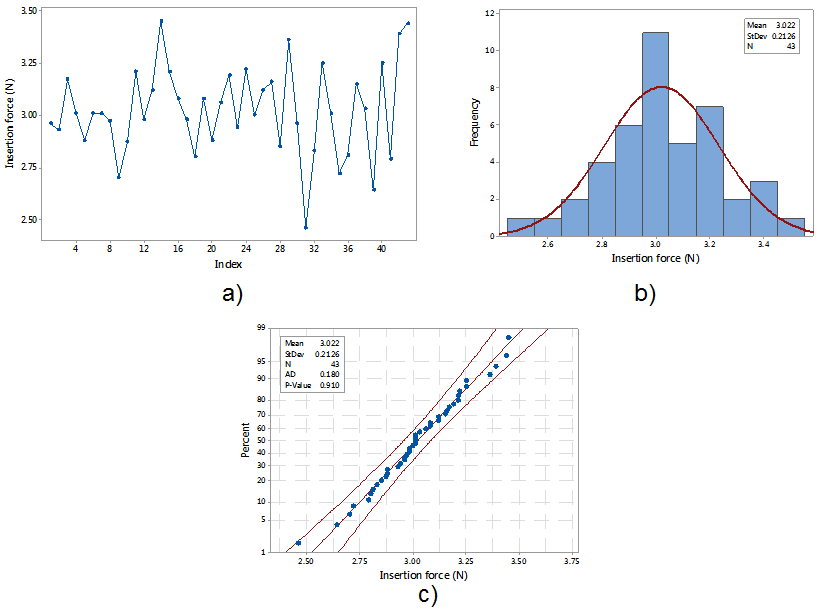
\includegraphics[height=11cm]{img/spc.PNG}
   \caption{Statstical}
 \label{fgr:PFS}
 \end{figure}
 
\subsubsection{Model prediction capability}

\subsubsection{BLF}

\newpage
\section{Discussion}
\subsection{Stopper movement minimization}
 
As briefly mentioned a specific requirement in this case are specific and for the URS it is specified for the stopper height.

URS/1 fdfdfs

Perhaps a better method of reducing plunger movement is by controlling the height of the plunger as well as the air space between the plunger and the sterile liquid. Studies conducted by Kinney et al. demonstrate that more plunger movement is expected as the air space between the plunger and the sterile liquid increases and as the height of the plunger decreases.

The resistance necessary for the snap-fit to occur is on the one hand provided by the air pressure compressed between liquid and rubber stopper, and on the other through friction of the stopper with the surrounding glass container. The combination of these two factors lead to

\subsubsection{Friction}
Silicone oil distribution should be as homogeneous as possible. Dry zones increase the friction. 	viscosity of Silicone oil and drug product  affect accorded to Formula 3 the friction. Interactions with the silicon layer through expedients are neglected in this work. But in the most practical cases, interactions between silicon oil layer on the barrel and product modify the friction[8]. Storage time affect the silicon amount between stopper and syringe barrel and the migration of silicone oil into the solution. The silicone oil flows out and friction increases over the time. Effect to $d_{oil}$. Silicon layer thickness depends proportional to silicon amount if the wetted surface is constant. Different layer thicknesses change the friction[16]. A thicker layer reduces the static friction. Effect to $d_{oil}$.
\begin{equation}
    d_{oil}=\frac{Silicon amount}{\rho_{oil} d_{barrel} \pi l_{barrel}}
    \end{equation}
Critical factor to BLF are: storage time, storage temperature, syringe size, supplier and silicone amount (show in Figure 11).
Critical for high BLF are a big stopper surface area, high storage temperatures, long storage times and a small silicone amount.
Disadvantage: High BLF can cause problems with the activation of the syringe.
Advantage: The stopper is less sensitive towards mechanical impacts. This means that a stopper movement should not occur.
Possible solutions to lowering the BLF are: Reducing the stopper surface area through a shortened stopper, increase the silicone amount or storage the syringe at 5 C.

\subsubsection{Critical factor contribution}


\subsubsection{Process solution}
\subsubsection{Design solution}

\subsection{Model / experiments}
These can be studied with experiments and model with a certain degree of accuracy. For example, a computer model will have exact dimensions while for the experiment there is always present a certain uncertainty caused by tolerances. 

Difficult to give precise quantitive statements


\subsection{2D - 3D model comparison}
Holistic simulation is too complex
Friction is a tricky business: 
Tribological studies
Silicon oil study
Multiple phenomena at once
The quicker the more interlinked they become

\subsection{Explicit - Static Comparison}


% Conclusion
\newpage
%\addcontentsline{toc}{section}{\protect\numberline{}{Conclusion}}
%\addtocontents{toc}{\vspace{.5\baselineskip}}
%\markright{Conclusion and Outlook}
\part{Conclusion and Outlook}
\section{Conclusion}
\section{Outlook}
Tribological studies
Silicon oil study

% Bibliografie
\newpage
\addtocontents{toc}{\vspace{.5\baselineskip}}
\addcontentsline{toc}{section}{\protect\numberline{}{References}}
\markright{Conclusion and Outlook}
\bibliography{arbeit}

% Nachwort (nicht zwingend)
\newpage
\addtocontents{toc}{\vspace{.5\baselineskip}}
\addcontentsline{toc}{section}{\protect\numberline{}{Afterword}}
\markright{Afterword}
\section*{Acknowledgment}
\label{s:Nachwort}

Nachwort, Danksagung und Ausblick.

% Anhang, falls benoetigt
\newpage
%\addtocontents{toc}{\vspace{.5\baselineskip}}
\appendix
\section{Appendix}
\label{s:Anhang}

\subsection{Anhang Kapitel}
\label{sec:umf_pot}

\begin{figure}[h]	
	\centering
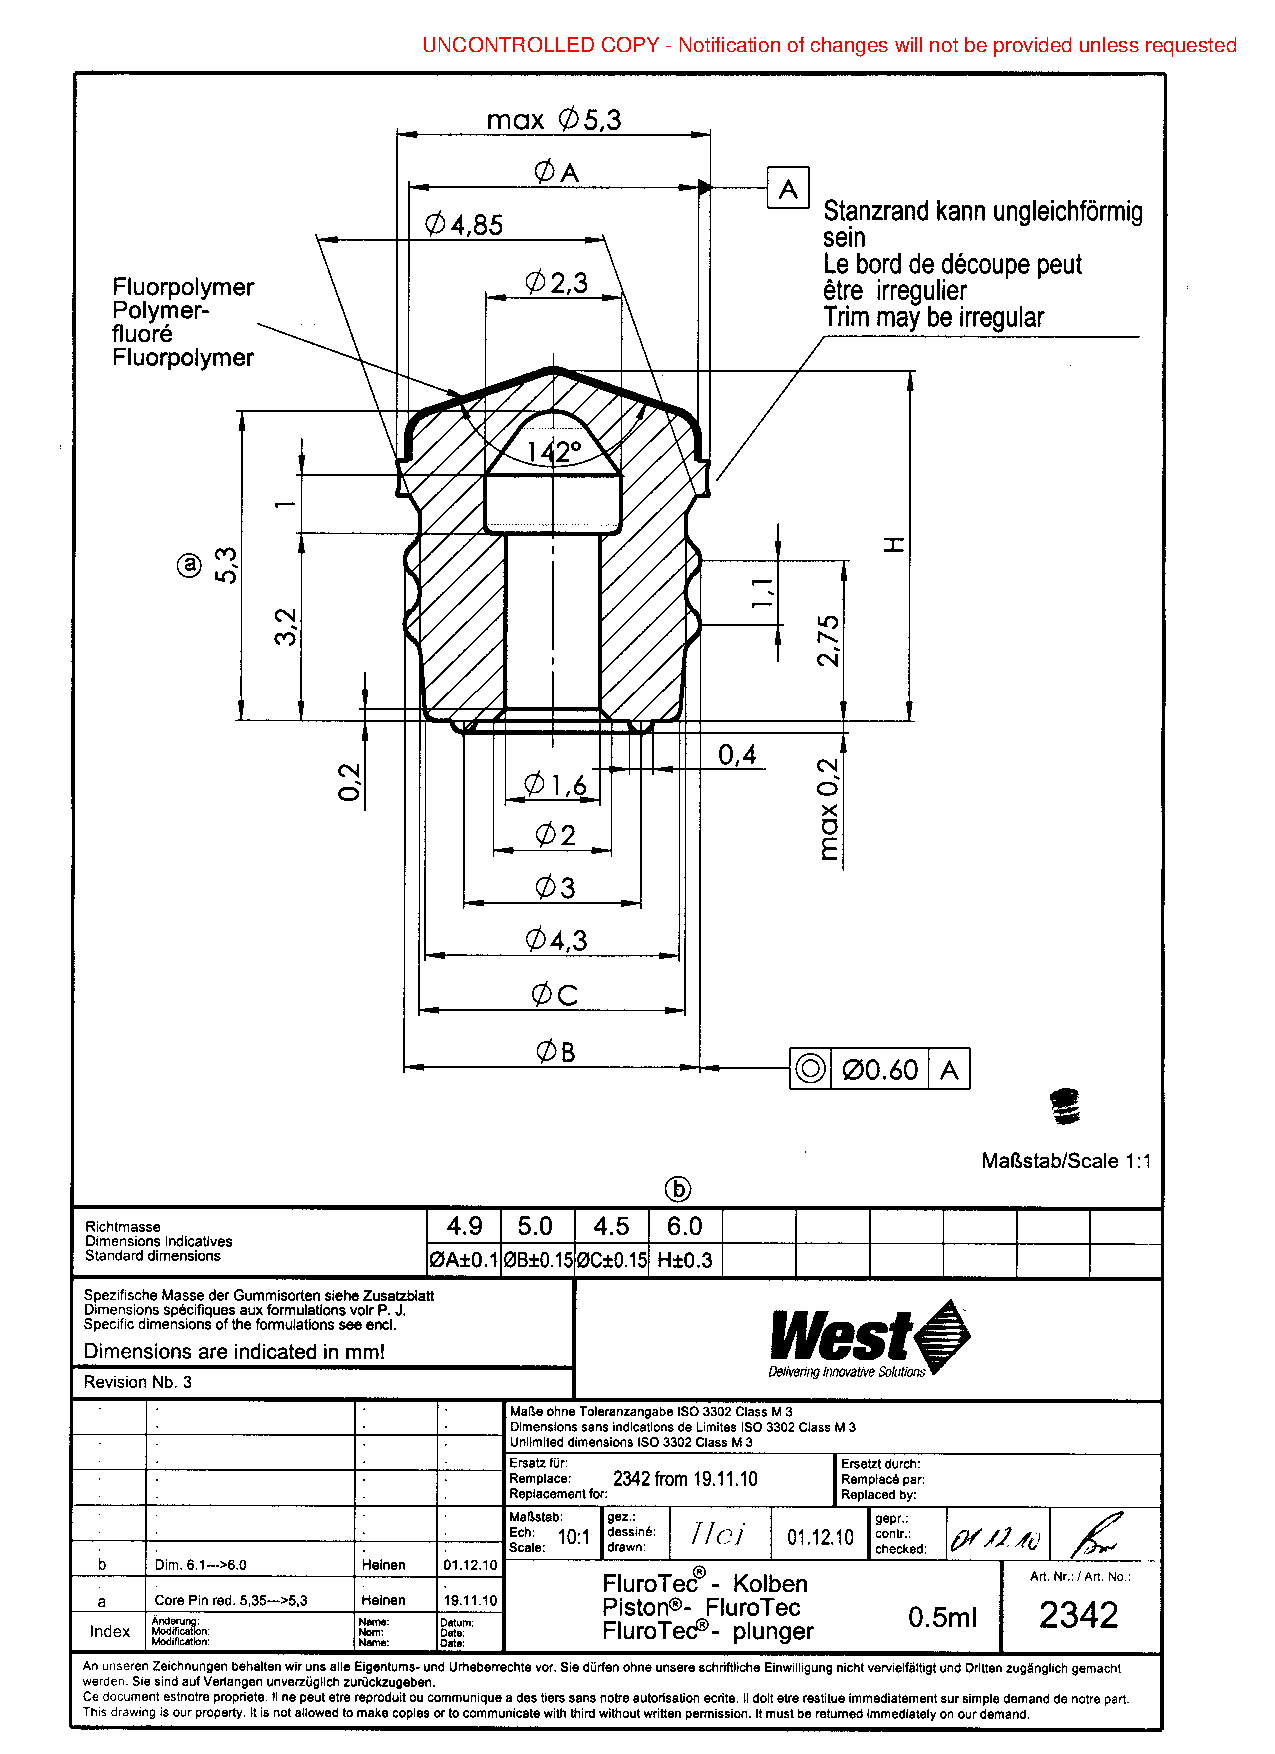
\includegraphics[height=6cm]{img/PS.pdf}
   \caption{Pre-filled Syringe.}
 \label{fgr:PFS}
\end{figure}

\begin{figure}[h]	
	\centering
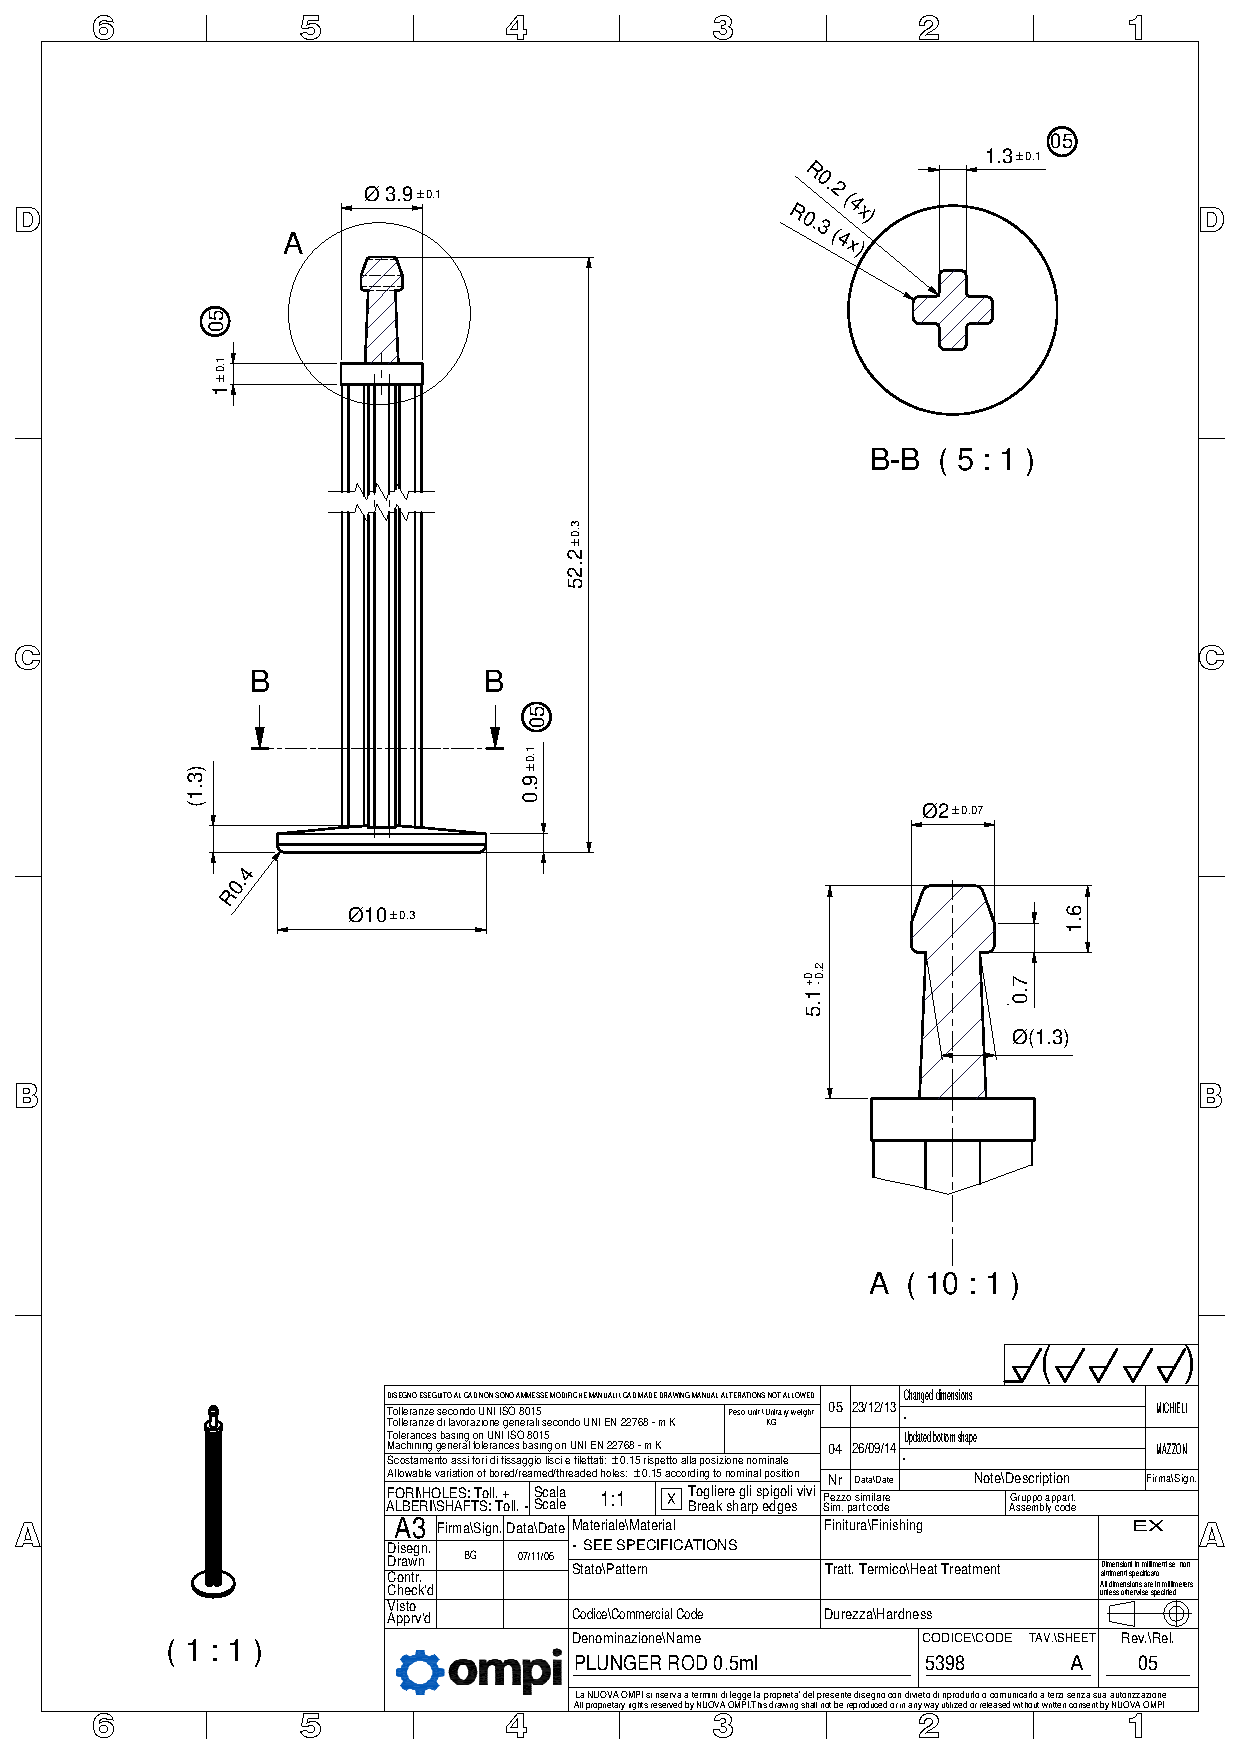
\includegraphics[height=6cm]{img/PR.pdf}
   \caption{Pre-filled Syringe.}
 \label{fgr:PFS}
\end{figure}
Hier kommt alles rein, was im Hauptteil der Arbeit keinen Platz mehr fand.



\end{document}

